\documentclass[openany]{ctexbook}
\usepackage{lmodern}
\usepackage{amssymb,amsmath}
\usepackage{ifxetex,ifluatex}
\usepackage{fixltx2e} % provides \textsubscript
\ifnum 0\ifxetex 1\fi\ifluatex 1\fi=0 % if pdftex
  \usepackage[T1]{fontenc}
  \usepackage[utf8]{inputenc}
\else % if luatex or xelatex
  \ifxetex
    \usepackage{xltxtra,xunicode}
  \else
    \usepackage{fontspec}
  \fi
  \defaultfontfeatures{Ligatures=TeX,Scale=MatchLowercase}
\fi
% use upquote if available, for straight quotes in verbatim environments
\IfFileExists{upquote.sty}{\usepackage{upquote}}{}
% use microtype if available
\IfFileExists{microtype.sty}{%
\usepackage{microtype}
\UseMicrotypeSet[protrusion]{basicmath} % disable protrusion for tt fonts
}{}
\usepackage[b5paper,tmargin=2.5cm,bmargin=2.5cm,lmargin=3.5cm,rmargin=2.5cm]{geometry}
\usepackage[unicode=true]{hyperref}
\hypersetup{
            pdftitle={They live in us},
            pdfauthor={范晓太,赵鹏},
            pdfborder={0 0 0},
            breaklinks=true}
\urlstyle{same}  % don't use monospace font for urls
\usepackage{longtable,booktabs}
% Fix footnotes in tables (requires footnote package)
\IfFileExists{footnote.sty}{\usepackage{footnote}\makesavenoteenv{long table}}{}
\IfFileExists{parskip.sty}{%
\usepackage{parskip}
}{% else
\setlength{\parindent}{0pt}
\setlength{\parskip}{6pt plus 2pt minus 1pt}
}
\setlength{\emergencystretch}{3em}  % prevent overfull lines
\providecommand{\tightlist}{%
  \setlength{\itemsep}{0pt}\setlength{\parskip}{0pt}}
\setcounter{secnumdepth}{5}
% Redefines (sub)paragraphs to behave more like sections
\ifx\paragraph\undefined\else
\let\oldparagraph\paragraph
\renewcommand{\paragraph}[1]{\oldparagraph{#1}\mbox{}}
\fi
\ifx\subparagraph\undefined\else
\let\oldsubparagraph\subparagraph
\renewcommand{\subparagraph}[1]{\oldsubparagraph{#1}\mbox{}}
\fi

% set default figure placement to htbp
\makeatletter
\def\fps@figure{htbp}
\makeatother

\usepackage{booktabs}
\usepackage{longtable}

\usepackage{framed,color}
\definecolor{shadecolor}{RGB}{248,248,248}

\renewcommand{\textfraction}{0.05}
\renewcommand{\topfraction}{0.8}
\renewcommand{\bottomfraction}{0.8}
\renewcommand{\floatpagefraction}{0.75}

\let\oldhref\href
\renewcommand{\href}[2]{#2\footnote{\url{#1}}}

\makeatletter
\newenvironment{kframe}{%
\medskip{}
\setlength{\fboxsep}{.8em}
 \def\at@end@of@kframe{}%
 \ifinner\ifhmode%
  \def\at@end@of@kframe{\end{minipage}}%
  \begin{minipage}{\columnwidth}%
 \fi\fi%
 \def\FrameCommand##1{\hskip\@totalleftmargin \hskip-\fboxsep
 \colorbox{shadecolor}{##1}\hskip-\fboxsep
     % There is no \\@totalrightmargin, so:
     \hskip-\linewidth \hskip-\@totalleftmargin \hskip\columnwidth}%
 \MakeFramed {\advance\hsize-\width
   \@totalleftmargin\z@ \linewidth\hsize
   \@setminipage}}%
 {\par\unskip\endMakeFramed%
 \at@end@of@kframe}
\makeatother


\usepackage{makeidx}
\makeindex

\urlstyle{tt}

\usepackage{amsthm}
\makeatletter
\def\thm@space@setup{%
  \thm@preskip=8pt plus 2pt minus 4pt
  \thm@postskip=\thm@preskip
}
\makeatother

\frontmatter

\title{They live in us}
\author{范晓太,赵鹏}
\date{2017-05-20}

\begin{document}
%%\maketitle
%
\begin{titlepage}
    \centering
    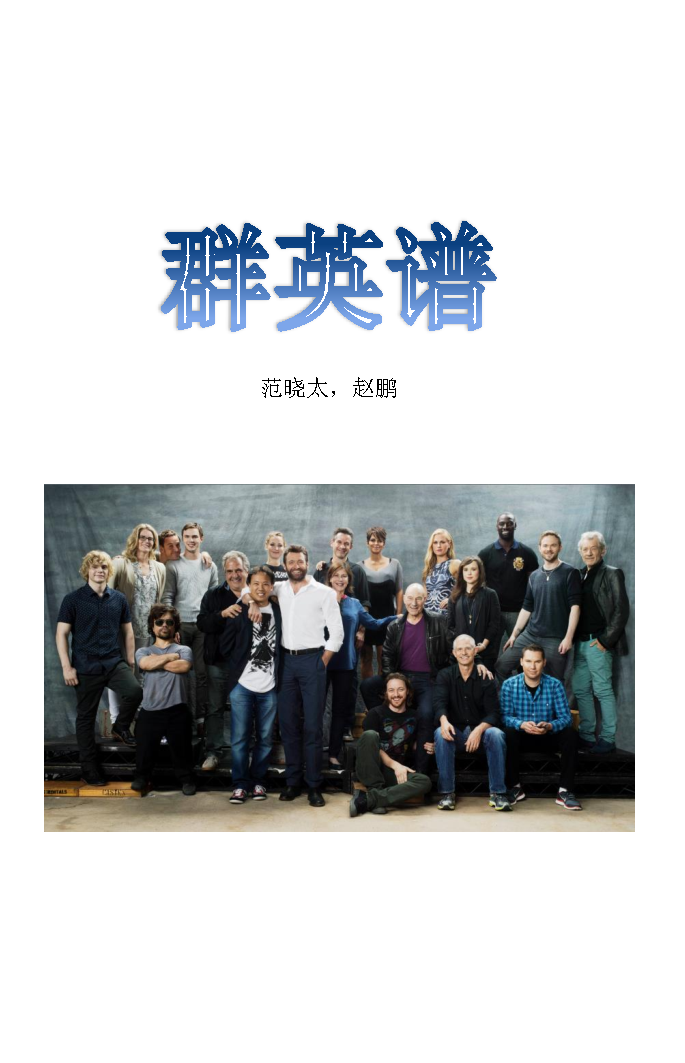
\includegraphics[width=\textwidth]{images/cover.pdf}
\end{titlepage}

\thispagestyle{empty}

\setlength{\abovedisplayskip}{-5pt}
\setlength{\abovedisplayshortskip}{-5pt}

{
\setcounter{tocdepth}{2}
\tableofcontents
}
\mainmatter

\part{群英谱}\label{qyp}

\part{1916疆班风采录}\label{part-1916}

\chapter*{不忘初心,执着梦想--告1916班全体同学书(一)}\label{letter1}
\addcontentsline{toc}{chapter}{不忘初心,执着梦想--告1916班全体同学书(一)}

公元2016年8月26日,艳阳高照。

新疆乌鲁木齐市第58中学,热闹异常。

国各地来疆接待新生的老师,风尘仆仆;新疆内高班的学子们齐聚一堂,心绪摇摇。

我的欣喜,你的羞赧,完美地融合在相顾一笑的对视之中。仿佛前世有个约定,让你我怦然心动。

从8月26日的第一次见面,到T198次列车上一天两夜的全程陪伴,在你们身上,我又看到了五年前刻骨铭心的一幕。

五年前,我积极响应党的号召,带着学校的嘱托,满怀一腔热情,克服一切困难,奔赴西部边陲,开展为期半年的援疆支教工作。在哈密这片广袤的热土上,在甘洒热血写春秋的同时,让我辗转反侧寤寐思服的,是那一双双真诚如镜,清澈如水,明亮如星的眼睛。无论是课上还是课下,都充满了对知识的渴盼,对先进的期待,对文明的希冀,对未来的想往。分别的时候,我对他们说:``但消屈指,何须回首,历历关山飞跃。哈密瓜甜,已成往事,最喜今朝柝。桃红李白,争春秀色,谱写千秋雅乐。筹他日,中原再会,共商举措。''

也许正是这一段特殊的经历,令我产生了一份儿特殊的感情,从而与不远千里来郑求学的西域的学子们结下了不解之缘。在以后的几年里,我所任教的班级中,从来都没有缺席过来自新疆的学生。他们尊敬师长,团结同学,能歌善舞,热心公益,刻苦勤奋,百折不挠的优秀品质,已然在中原大地上生根、发芽、开花、结果。

从乌鲁木齐到郑州,三千多公里的路程,一天两夜的长途跋涉,同学们饱受颠簸之苦。但是,没有一个人畏惧,更没有一个人退缩。为什么?因为每一个同学心中都有一个灿烂的梦想。梦想的内容和形式可能会因人而异,但梦想的根由和初心,却大致相同,那就是对现实的改造和对理想的憧憬。因而,这梦想就成为了鼓舞我们勇往直前的滔滔动力,招引我们奋勇向前的熊熊火炬。

到郑州十一中后,同学们来不及抚去身上的尘土,擦去脸上的倦意,就投入了紧张而艰苦的军训。五天,时间虽然短促,意义却异常深远。这一点,在以后的学习生活中你们会有深切的体会。我想说的是,军训过程中,咱们同学都体现出了一不怕苦,二不怕死的军人品质和精神,践行着流血流汗不流泪的坚毅与刚强。因为,我们每一个同学都明白,我们的肩上有一副沉甸甸的担子,这担子,就是责任。我们带着父老乡亲的厚望,同学朋友的期许,国家民族的寄托,从五湖四海,为了一个共同的目标,走到这里来了。

同学们,我们疆班的全体任课老师已经做好了充分的准备,将会以眷眷之心为牵引,诱思探究为法器,课里课外为阵地,鞠躬尽瘁,死而后已;疆班的全体任课老师也相信,同学们一定会用拳拳之心为激励,健康成长为目的,勤奋刻苦为武器,生生不息,孜孜不止。

我多想饮一杯冰水稳定一下情绪,跳动的脉搏瞬间颠覆了我的思虑;遥想当年倒拔垂杨柳的钢筋铁骨,怎能眼睁睁看着彩霞阒然地遁去。

火光在前,胜利在前。同学们,让我们携起手来,不忘初心,执着梦想,继往开来,奋勇前进吧

--- 2016、9、5

\chapter*{祝1916班九月份生日的同学生日快乐}\label{birthday9}
\addcontentsline{toc}{chapter}{祝1916班九月份生日的同学生日快乐}

古丽扎巴天上虹,和风细雨妙玲珑。瘦红肥绿一牵手,流瀑飞泉唱大同。

(古丽扎巴,9月12日。)

艾则麦提江,力能把鼎扛。若问何能尔?志在巧安邦。

(艾则麦提江,9月13日。)

唐人自古洒豪情,静夜深思揽月明。不到黄河心不死,凡夫俗子靠边行。

(唐静,9月16日。)

人小心高木尔都,郑州求学绘蓝图。四年展翅晴空去,横绝红尘抱玉壶。

(木尔都,9月24日。)

浩浩苍穹何处寻?锦囊妙计我来擒。多谋善断人人酽,才调横空降雨林。

(赵浩锦,9月26日。)

巴登才次克,举世有无双?中外存心底,古今入右窗。天高飞国梦,海阔跃昆腔。掬挹黄河水,澄清十九缸。

(巴登才次克,9月29日。)

\chapter*{钢 铁 意 志 木 尔 都}\label{muerdu}
\addcontentsline{toc}{chapter}{钢 铁 意 志 木 尔 都}

2016年9月30日下午一点五十分左右,在郑州市第十一中学玉辉楼一楼东侧的观察室里,我见到了木尔都。此时此刻,距离玉辉楼不足百米的操场上一片沸腾,呐喊声震耳欲聋。同学们都用尽了吃奶的力气,在为自己班的运动员加油助威。学校第85届秋季田径运动会最后一个项目4x100米,正在如火如荼地进行。然而,热闹是他们的,我的心思全在这一间冷冷清清的小屋里。

当内派老师胥明推开房门的瞬间,我还以为没人呢。仔细看时,才发现蜷缩成一个单薄小团的木尔都,趴在东边靠近南窗户的木板床上,身上盖着一件灰色秋装,头发凌乱,面色赤红,好像睡觉的样子。就这一瞥,一股酸涩涌上鼻尖,一汪咸水集聚眼底。

上午九点钟前后,是女子800米赛事,木尔都代表班级出战。可是,就在接近终点的跑道上,她摔倒了。而且,一直站不起来。120来了,做了简单的检查,说,没事,再观察观察。于是,身材矮小,几近虚脱的木尔都,被人扛进了这间只有几张硬板床的小屋里。--遗憾的是,这些情况是我到了小屋,见了木尔都之后才知道的。作为班主任,有一种失职的愧疚感,像毒蛇一样啮噬着我的心。

我不知道该怎样表达我的歉意,就把手中的冰激凌作为慰问品,放在了她的床前。环顾四周,床头,有好友倒在暖壶盖里的热水;床前的椅子上,有好友从餐厅代买的一杯奶茶,一卷油饼;傍边,还有一截吃剩的奥利奥。很显然,木尔都还没有吃午饭。后来,在交谈中又知道,木尔都早饭都没有吃。因为要值日,就取消了吃早饭的时间;因为要参加比赛,就随便吃了几片奥利奥。这几片奥利奥,就成了她奔跑800米冲刺奖牌为班争光的所有食粮。

木尔都,你为了班级的荣誉,居然这样的拼命!

木尔都,你为了集体的利益,竟然如此的疯狂!

木尔都,你是坚强的,坚强得有如顶天立地的共产党员!

木尔都,你是威武的,威武得浑似冲锋陷阵的勇猛斗士!

在20多分钟的谈话过程中,木尔都一直咳嗽,这让她赤红的脸颊有时会发紫。可能是因为摔倒后被救助时喝了一些凉水,引起的肺部的不适。这也许是她没有能够吃下午饭的原因。然而,木尔都始终都以微笑的面容对我,偶尔也会对自己的失误报以羞赧,甚至自责。她一直在强调,自己不应该是这样子的,以前训练时也有过类似情况的发生,但是,这一次绝对不应该再出此类的事情的。

她说话时,我能够看得见她的眼睛里闪烁着的晶莹,可是,她始终没有让那闪烁的晶莹聚集成露珠而滑落出来。我也能够深刻地感受到,闪烁的晶莹里所包含着的苦涩的味道,和隐寓着的钢铁般的意志。我佩服她的刚强,却担心她的腿。因为摆在我眼前的不可否认的事实是,她的左腿不能动弹,抬不起来。木尔都笑笑,说,没事的,没事的。我让她活动活动给我看,她试了几试,一边用双手按摩推拿,一边用双手将左腿搬起来,以达到能够屈伸的目的。最后她的左腿终于能够自己活动了。

我回到操场,找了巴登和晁文秀来陪她说话,避免孤独和寂寞给她带来二次伤害。

运动会结束后,我将要回家的时候,又到观察室去看她,却已是人去屋空。正像她所说的那样,没事的,我会好起来的,后天还要去少林寺呢!

这正是:

铁骨钢筋木尔都,历经磨难得珍珠。

从容走过人间道,笑傲江湖不服输。

2016、9、30

\chapter*{时间的去向与归宿--告1916班全体同学书(二)}\label{letter2}
\addcontentsline{toc}{chapter}{时间的去向与归宿--告1916班全体同学书(二)}

曾几何时,一曲《时间都去哪儿了》,感动了多少有情人,催下了多少辛酸泪,唤回了多少不归客,惊醒了多少逐梦者,真可谓功不可没。尤其值得称赞的是,这首歌随着时间的推移在不断地发酵,升华,犹如跌荡开去的层层涟漪,传播着神奇的蝴蝶效应。只要歌声响起,就会引发人们对过往时光的无穷的思忖,对现实状况的无限的追问,以及对美好未来的无尽的憧憬。

眨眼之间,我们已经在古老的商都郑州生活学习了一月有余,六千里外的挂念与期盼,可曾激起你对时间的去向与归宿的思考?我相信,每一个同学的心中,都会有一个只属于自己的答案。惆怅抑或欢喜,平淡抑或激昂,大概就是纷繁答案的情绪化表达形式。但,无论怎样,时间在属于芸芸众生的同时,也属于我们每一个个体,而且,它已在我们每一个人的身上烙下了不可磨灭的印记。

时间就像一个调皮淘神的顽童,就在我们端坐在教室里,映着明亮的灯光,专心致志地读书的时候,它悄无声息地爬上我们的额头,沿着眉梢发际上的光亮,做贼似的,慢慢地,慢慢地滑动,唯恐被发现后,落得像讨人厌的蚊子一样的下场。好在它的轻功相当了得,再加上我们的注意力完全被书里的内容吸引住了,根本没有觉察到孙悟空在西天柱上留下的痕迹。它静悄悄地滑过,自以为神不知鬼不觉。我们的大度,宽容了它的戏谑。

时间就像一个神情庄重的长者,就在我们全神贯注地望着黑板,一边聆听老师的讲解,一边下意识地做着笔记的时候,它凛然如君王一般,目光炯炯地巡视着我们每一张朝气蓬勃的脸,那充满正道的眼神,仿佛疲劳倦怠不安心之探测仪,迅速而又细致地扫过我们张弛有度的脉搏,记录下分分秒秒的心跳,存入分门别类因人而异的档案。我们的病例,全在它的数据库里。也许有一天,它会用这些琐碎而翔实的资料,与我们算总账,一笔一笔。

时间就像一个雄赳赳气昂昂擅长跋涉的机器人,所到之处,没有什么可以阻挡;所过之处,也没有什么值得留恋。它始终如一地保持着匀速运动,步履之坚毅,步伐之果断,为有史以来之唯一。真真正正的冷血,地地道道的无情。它用固有的漠然之态度、淡然之风格、木然之表情、坦然之心理,缔造了万物生命的珍贵,也成就了万物生命的辉煌。它不仅让生命的光辉像日月一样灿烂,而且让生命的质量像峰峦一样厚重。

富兰克林说:``你热爱生命吗?那么就别浪费时间,因为时间是组成生命的材料。''由此可见,时间是生命的计算器,而生命则是时间的量杯。生命因时间而恢弘着舍我其谁的勃发英气,时间因生命而彰显出惟我独尊的称霸豪情。我们既是时间的无私的见证者和实践者,又是生命的狂热的爱好者和追随者。在我们心中,每一分每一秒都承载着生命的价值和意义,每一时每一刻都创造着生命的奇迹和壮举。

于是,我们用朴实无华的一举一动,一颦一笑,让不可一世的时间无法遁形,无处藏身,无计可施。不信?你看:时间,就在我们挺拔坚毅的腰板里--这叫力度;时间,就在我们风风火火的脚步里--这叫强度;时间,就在我们会心的微笑里--这叫热度;时间,就在我们求知若渴的眼睛里--这叫浓度;时间,就在我们沙沙沙沙的奋笔疾书里--这叫风度;时间,就在我们冥思苦想的紧蹙的眉头里--这叫态度\ldots{}\ldots{}

庄子曰:``吾生也有涯,而知也无涯。以有涯随无涯,殆已。''在历史的长河中,我们用我们短暂的几乎微乎其微的生命,丈量着汹涌向前滔滔不归的时间的长度,这是怎样的一种伟大呀!我们有什么理由不举起右臂,向我们自己献上庄重的--敬礼?!

2016、10、5

\chapter*{祝1916班十月份生日的同学生日快乐}\label{birthday10}
\addcontentsline{toc}{chapter}{祝1916班十月份生日的同学生日快乐}

欧力加斯棒小伙,载歌载舞到中州。中州古韵惹人醉,不负平生对月钩。

欧力加斯(10、7)

存肄郑州十一中, 微而具体不言功。 今朝勤苦明朝福, 雨过天晴沐惠风。

冶存微(10、16)

聪明颖脱世间奇,林木葱葱情敢移。锁住阳光争上游,目标坚定意淋漓。

林聪颖(10、19)

阿鹊谁来说我亲? 瓦当滴落九成新。 古来不改乡音韵, 丽泽殷殷问渡津。

阿瓦古丽(10、20)

大任落肩古丽江,情真意切坐寒窗。曾经目不窥园日,只为今朝龙虎降。

古丽江(10、23)

\chapter*{祝1916班十一月份生日的同学生日快乐}\label{birthday11}
\addcontentsline{toc}{chapter}{祝1916班十一月份生日的同学生日快乐}

马如流水耳盈玲,欢乐不教白日暝。学海滔滔冲浪去,一书一笔一亭亭。

(马玲,11月2日)

高瀑飞泉祥瑞生,鹊桥壮丽向天横。五光十色心弦扣,正值华年飞碧甍。

(高泉瑞,11月14日)

深藏不露是罗强,睥睨群雄意气扬。四两千斤非技巧,灵犀彩凤共翱翔。

(罗强,11月15日)

文质彬彬卓荦人,胸中有竹太阳自然新。条分缕析乱麻斩,秣马厉兵绝尘。

(符文卓,11月19日)

薛珂喜静爱埋头,万卷攻坚上层楼。不见闻鸡起舞者,横扫天下壮志酬。

薛珂(10、26)

\chapter*{窗外,那一双眼睛--告1916班全体同学书(三)}\label{letter3}
\addcontentsline{toc}{chapter}{窗外,那一双眼睛--告1916班全体同学书(三)}

``窗外,有一双阴冷的眼睛,时不时会射出刺骨的寒光,常常让人陡生如履薄冰如临深渊之悸,顿生如芒在背如坐针毡之慨。如果不是拥有一颗砰砰跳动的充满活力的心脏,如果没有虽千万人吾往矣的强大的心理承受力,绝对抵挡不了这一天之中数个小时的无量次的暗箭的攒射。\ldots{}\ldots{}''

``窗外,有一双温暖的眼睛,时不时送过来拂面的熏风,常常让我们拥有如登春台如获至珍的幸福感,享受如沐春风如饮甘霖的快乐体验。如果不是怀揣着一颗充满了深情的大爱之心,如果没有春蚕到死丝方尽的无私的乐于奉献的精神,绝对不会一天天几乎把所有的时间都花费在我们这群不让人省心的孩子身上。\ldots{}\ldots{}''

这是针对同一种现象而表现出来的截然不同的两种看法。因为它来源于同一时段的同一本``教室日志'',所以有理由认为这是同学们的真实心理写照。仁者见仁,智者见智,看法不同,自是常理。但从心理学的角度来看,它反映的却是两种截然相反的处世态度:一种是积极的,通常叫做阳光型;一种是消极的,按照惯例叫做阴暗型。

我上中学的时候,也最讨厌老班趴在后窗户偷窥我们的一举一动一言一行一颦一笑。原因很简单:我们需要绝对的隐私,而老班却是一个``偷窥狂''。因为她常戴一副黑边眼镜,被同学们私下里戏称为``国宝眼镜蛇''。(现在``眼镜蛇''变成了对全体老师的官称,可见社会在进步。可惜我不戴眼镜。)后来,她知道了,一度神情沮丧,好像得了什么不治之症。吓得我们都自发地准备向她承认错误,乞求她的惩罚。终于有一天,她压抑了多日的情绪爆发了。

那是班会时间,太阳早已不见了踪影,她还在滔滔不绝,声嘶力竭地申诉着。她像一个受了很大委屈的孩子,声音有些发抖,讲话没有条理,眼眶是红的,眼泪却始终没有掉下来。她慷慨激昂,我胆战心惊,所以,她说的什么,回家后全然忘怀。但是,从那以后,我不再排斥老班的``偷窥'',因为我奇妙地觉得一夜之间自己长大了,懂事了,成熟了。再看其他同学,也和我一样,仿佛玩魔术一下子变了一个人似的。

前些年,有一首歌很流行,歌名叫做《长大后我就成了你》。我不敢说歌词里说的就是我,事实是,我大学一毕业,就登上讲台,做了一名向往已久的教师。在提及往事时,曾经和满脸稚气的孩子们约定:绝不``偷窥''。然而,半个学期过后,班会时间,我当众宣布,取消了先前的约定。原因大家心知肚明,所以没有一个反对的。

教室前后两扇门上的一尺见方的小玻璃窗的最大的功用绝非为了采光,而是为了便于观察,而且主要是为了便于观察里面的动静和异常情况,以便及时作出处理,以免贻误时机。而观察者通常是班主任和值班老师,其中,班主任的几率最高,可达百分之九十九。那么,班主任``偷窥''的心态到底是什么,你们懂吗?教室是干什么的,你们做到了吗?不远千里到郑州为什么来的,你们还记得吗?国家的厚爱与付出,你们感恩吗?父母的牵挂与期盼,你们领情吗?除了吃饱穿暖就是玩得痛快,你们心安理得吗?

我国有句谚语说得好:``为人不做亏心事,半夜不怕鬼敲门。''班主任的``偷窥'',其实不是要抓什么典型,而是习惯的巡视,就像菩萨,一心想着要施救于民。千万不要以小人之心,度君子之腹。子曰:``君子坦荡荡,小人长戚戚。''

请记住:心虚者看到的是监督与不信任,坦荡者看到的是关爱和呕心沥血。

我可以``如烟往事俱忘却,心底无私天地宽。''你们呢?

2016、11、1

\chapter*{\texorpdfstring{我们是``特种兵''(朗诵稿)--告1916班全体同学书(四)}{我们是特种兵(朗诵稿)--告1916班全体同学书(四)}}\label{letter4}
\addcontentsline{toc}{chapter}{我们是``特种兵''(朗诵稿)--告1916班全体同学书(四)}

\textbf{第一章 时时引领望天末,心随潮水共悠悠}

\begin{verbatim}
【旁白】曾几何时,羞怯的面容上,满是清晨丽日般的渴盼。还有那一双双眸子,无私地打开了心灵窗户的两扇;浑似镶嵌在碧空里的宝石,闪耀着谜一样的梦幻。

那时那刻随流水,此情此景贮心间。
\end{verbatim}

男1:我们是特种兵,来自遥远的天山。

女1:天山的广阔,栖息着王母娘娘的心愿。

女2:心愿里的故事,讲述了整整五千年;

男2:五千年,发酵的微醺,醉红了东方的蓝天。

男1:从天山到嵩山的距离,一寸一刀,都刻在了时间的魔盘。

女1:一百个日日夜夜,酿出了几多苦辣酸甜。

男2:白天的高强度学习,我们任劳任怨;夜间的无限思念,有谁能够说得完全?

女2:家乡的空气成了梦里的贪婪,亲人的笑脸镌进了记忆的狂欢。

女1:我们只有十五岁,稚嫩的心灵却写满了拼搏的信笺。

男2:我们只有十五岁,纤弱的肩膀早已承载了未来的重担。

男1:长辈的嘱托我们不会忘记,无论前方有多少沟沟坎坎。

女2:同龄人的艳羡是挥舞的长鞭,不管风骤雨狂始终咬紧牙关。

女1:我们已经十五岁,坚强的心灵足以翻越命运的苦难。

男1:我们已经十五岁,硬朗的肩膀能够载得起任何挑战。

女2:老师的话语时刻响在耳畔,吸引我们的何啻知识的烂漫!

男2:同伴们的互帮互助亲密无间,构筑成一道无往不胜的烽火线!

男1:我们是特种兵,注定了生命轨迹的曲曲弯弯。

女1:我们是特种兵,筑成了生命色彩的斑斑斓斓。

男2:我们是特种兵,贮藏了生命内涵的灿灿烂烂。

女2:我们是特种兵,铸就了生命姿态的翩翩跹跹。

\textbf{第二章 琉璃玉匣吐莲花,错镂金杯映明月}

\begin{verbatim}
【旁白】多少年后,何须繁复的胶片,更不必检索档案;只要说一声--我想看,顷刻间烟花灿烂。激动时刻的雀跃狂欢,沉醉阶段的星斗阑珊;故事里的扣人心弦,童话世界的五千年。
\end{verbatim}

女1:你是天山雪峰上,滚落的一块冰坨。在无边的夜空里,奋力碾过,跌跌撞撞、坎坎坷坷。

女2:圆了,清了,亮了,终于呈现出玉盘一个。

男1:苍穹如幕,为你搭建浩瀚舞榭。你怀抱无弦琴,弹奏起心灵的歌。

男2:一颗流星,从你的心弦滑落,栖在我的心头,慢慢叙说\ldots{}\ldots{}

(女声合)经历了风花雪月,看惯了生离死别,就不再把网络,拼命地挣脱。

(男声合)静静地等待,悄悄地磋磨,让世界沉浸在,举首的祝贺。

女1:你还记得巴里坤山口的风吗?神情豪迈飞速转动着发电的扇叶。

男1:你还记得淖毛湖的胡杨林吗?静穆地演绎着三千年不倒的壮烈。

女2:看不够的塔里木河呀,惊诧于地球的耳朵。

男2:吐鲁番的葡萄哟,达坂城姑娘动情的歌。

男1:冬不拉跳跃在指尖的魂魄,可曾融化过峰峦叠嶂的雪?

女1:十二木卡姆回荡的旋律,瞬间征服了林林总总的小家大国。

男2、喀纳斯时隐时现的怪魔,能否解开我们是从哪里来的迷惑?

女2:克拉玛依星罗棋布的油井,霎时完成了魔鬼城堡的碣。

女1:当旭日冉冉升起的时候,我们挺身而出,不让光阴错过。

男1:当烈日炎炎似火的时候,我们知难而上,不教岁月蹉跎。

女2:当彩霞映红大漠的时候,我们信心百倍走向沙场,势不可遏。

男2:当银鹰掠过山巅的时候,我们高举着胜利的旗帜,雄心勃勃。

男1:我们是特种兵,注定了生命轨迹的坎坎坷坷。

女1:我们是特种兵,筑成了生命色彩的斑斑驳驳。

男2:我们是特种兵,贮藏了生命内涵的轰轰烈烈。

女2:我们是特种兵,铸就了生命姿态的风风火火。

\textbf{第三章 赤橙黄绿青蓝紫,谁持彩练当空舞}

\begin{verbatim}
【旁白】涌泉的眷眷,滴水的拳拳,从来没有对等的路线。父母的一声唤,摇曳着无穷无尽的烂漫。子女的一个吻,留下的传说说不完。
\end{verbatim}

男1:我多想说再见是为了再见,轻轻地挥手摇落美好的祝愿;

女1:千山万水隔不断滚烫的思念,繁星点点汇成汪洋的企盼。

男2:我多想化作一眼甘泉,经年累月滋润你干涸的心田;

女2:春天来花儿竞相开放,我们相逢在朝气蓬勃的花园!

男2:尊敬的爸爸,孩儿立志出乡关,不破楼兰终不还。

女2:亲爱的妈妈,生当人杰死亦雄,钢铁长城花木兰。

女1:天山的雪莲,嵩山的少林,引领我们绕指百炼。

男1:西域的广袤,中州的厚重,敦促我们力可拔山。

男2:还有什么比高山更坚毅的吗?我们站在高山之巅。

女1:还有什么比流水更欢快的吗?我们是流水中的仙。

男1:刚柔相济,百折不挠,这就是我们的品质,我们的情感。

女2:真的猛士的哀痛与幸福,我们用行动再谱新篇。

男1:殷墟的文字,东京的梦华,彰显着人类的智慧与才干!

女1:洛阳牡丹国,清明上河图,蕴藏着世界的文明和发展。

男2:尊敬的爸爸,请您自豪地说:我儿子让我挺直了腰板!

女2:亲爱的妈妈,请您放心地睡:梦里梦外都是一样的艳阳天。

男1:我们是特种兵,注定了生命轨迹的曲曲弯弯。

女1:我们是特种兵,筑成了生命色彩的斑斑斓斓。

男2:我们是特种兵,贮藏了生命内涵的灿灿烂烂。

女2:我们是特种兵,铸就了生命姿态的翩翩跹跹。

\textbf{第四章 踏遍青山人未老,风景这边独好}

\begin{verbatim}
【旁白】前世今生的魔咒,钉在襟间的钮扣;天山雪水的涓涓细流,人间至真至纯的美酒。忖一忖,风霜涤尽千番垢;聆一聆,醉卧云头。
\end{verbatim}

女1:烟霞深处的一抹心灵,偶然的机遇,幻化成几朵娇艳的精英。

男1:不用端详就知道,哪些花朵,有多少次冲破了梦的田埂。

男2:梦乡的滋味,蒸腾后又缭绕凝聚,既沉重,又轻盈。

女2:我不说,你也明白--我们是特种兵。

男1:我们是特种兵,因为我们肩负着特殊的使命。

女1:我们肩负着特殊的使命,所以我们是特种兵。

女2:特种兵自有特种兵的景行。

男2:特种兵自有特种兵的秉性。

男1:痛苦和劳累,是锻造屠龙宝剑的炉火腾腾。

女2:鲜血与汗水,是淬炼剑锋的琼浆一泓。

男2:十年一剑,星光闪烁的时候,长城内外集聚着远跖的鲲鹏。

女1:来日试看,东风劲吹的时候,大江南北会响起奋进的号声。

男1:我们是特种兵,注定了生命轨迹的崚崚嶒嶒。

女1:我们是特种兵,筑成了生命色彩的郁郁青青。

男2:我们是特种兵,贮藏了生命内涵的晶晶莹莹。

女2:我们是特种兵,铸就了生命姿态的纵纵横横。

2016、11、15---17

\chapter*{祝1916班十二月份生日的同学生日快乐}\label{birthday12}
\addcontentsline{toc}{chapter}{祝1916班十二月份生日的同学生日快乐}

月洒佳辉露洒珠,珠圆玉润唱腔殊。殊途亦有同归理,理所应当情不孤。

(王佳辉,12月4日)

韩雪建瓴高屋巅,云飞樯动过婵娟。婵娟激奋舞长袖,歆慕家乡不夜天。

(韩雪,12月9日)

卡片随身好习惯, 地球围着太阳转。 尔馨定律莫雌黄, 亚匹青衿情愫炫。

(卡迪尔亚,12月21日)

平生好学郑州跫,西望天山意万重。一颗红心明宇宙,光阴飞度自从容。

(吴明宇,12月29日)

\chapter*{\texorpdfstring{渔家傲·祝1916``雏凤清音''赛团凯旋}{渔家傲·祝1916雏凤清音赛团凯旋}}\label{sing}
\addcontentsline{toc}{chapter}{渔家傲·祝1916``雏凤清音''赛团凯旋}

雏凤清音情烂烂,博观楼里声声唤。济济一堂歌伟岸。须细看,人间少有时间段。

一六英豪伸铁腕,摩拳擦掌灵光灿。六杰挺身来夺冠。天浩瀚,群星闪烁苍穹幔。

2016、12、2

\chapter*{随缘·随喜·随心--告1916班全体同学书(五)}\label{letter5}
\addcontentsline{toc}{chapter}{随缘·随喜·随心--告1916班全体同学书(五)}

我不信命,BUT,我信缘。

``缘''是什么东东?不好诠释,BUT,好理解,即所谓``只可意会不可言传''者,浓缩成三个字:``你懂得''。

2016年8月26日,是我们生命长河中浪花泛起的一个别样的萼片,这个萼片勾画和渲染了你和我从今而后的生命的式样与色彩;新疆乌鲁木齐市第58中,是我们人生驿站里生火打尖的一出别致的绳结,这个绳结紧紧地拴住了我和你关于人生轨迹的走势与脉络。

这就是``缘''。--无形却有力量,无味却有气场的``缘''。

特别的时间,特定的地点,特出的人群,为了特有的使命,建立起特种的关系,从而产生特殊的感情,携手并肩共创特异的事业。一切都是那么的顺风顺水,水到渠成。没有一丝一毫的刻意,没有一丝一毫的斧凿。就像春来花开,秋来花落,不喜不悲,不慌不忙,不动声色,不惧炎凉。

佛教认为由于外界事物的刺激而使身心受到感触叫作``缘'',因其缘而发生动作称``随缘''。``缘''可遇而不可求。既然``缘''来了,那就安安心心地``随''着吧。

于是,第一个闯入镜头的太外茹柯,积极参与公益卸货的李正一,第一个排队领取食物的古丽扎巴,候车大厅里接受采访的马玲,火车上突然牙疼的赛力买,餐车厢中大摆``大''字的韩凯毅,会下象棋的唐静,主动让座的木尔都,莞尔的唐永秀,赧然的林聪颖\ldots{}\ldots{}还有第一个代表疆班学生发言的提拉热,勇挑班级管理重担的韩雪,迎着风浪前进的古丽江,轻松一跃即获得高一年级跳高冠军的欧力加斯,发不清``c''和``s''音的苏力谈,被封为男神学霸的王海旭,羞怯而又坚毅的奥斯曼江\ldots{}\ldots{}

从那一个特别的时刻起,我们就像是一同浮沉在特定江河段中的苇叶,腾挪跌宕,抑扬顿挫,遗世独立,羽化登仙。沿途的风景因我们的漂流而显得光彩夺目,青春焕发,仿佛被什么附了体的精灵,刹那间富有了只争朝夕的雄伟气魄,将所有的美丽尽情地绽放,把深邃的魅力发挥到极致。这便是``随喜''。随喜者,见他人行善而生欢喜也。

随喜,作为一种赞同别人而不嫉妒别人的礼仪习惯,存在于生活的方方面面,存储在生活的点点滴滴。当看到他人某方面做得比自己好的时候,我们会情不自禁地予以赞扬,并进而向他人学习,通过相互帮助相互鼓励的方式,使自己也得到提高,从而达到双赢之境界。是谓惺惺相惜,肝胆相照,同声相应,同气相求。

当一切的一切都似乎顺理成章的时候,我们再回过头来上下端详里外审视一下我们并肩作战冲锋陷阵的队伍--郑州十一中1916班。此班由18个男生和36个女生组成,共54人。54,正好是一副完完整整的扑克牌数目。如果说正副班长就是牌中的大小王的话,那么,其余的52个人,可以均分为四个组,每组又可均分为黑、红、梅、方四种花色,各种花色与数字和英文字母的组合,又都起着独一无二不可替代的作用。

于是,一年365天的对应,包括闰年的变数,在这个风雨同舟同舟共济的班集体里,都有了归宿,既落实到位,专职专责;又灵活多变,花样翻新。分分秒秒的跋涉印迹,时时刻刻的蜜蜂采集,潮涨潮落的岁月记忆,云卷云舒的蓝图欣喜,极视听之娱,畅幽情之乐。每一颗跳动的心,随着自己的意愿,划出一道道绚丽的彩虹,妆扮着寂寥的长空。目之所遇,耳之所得,情之所动,念之所在,合于《桑林》之舞,乃中《经首》之会,是一首地地道道的足以唱彻宇内宙外的歌。是随心之谓也。

随缘-随喜-随心,人间至乐者也!吾与子之所共适。

2016、12、26

\chapter*{祝1月份和7月份生日的同学生日快乐}\label{birthday1}
\addcontentsline{toc}{chapter}{祝1月份和7月份生日的同学生日快乐}

别力扎提游太空, 千山万水贮心中。 冰消雪化春来日, 唤友呼朋再用功。

(别力扎提 1、1)

麦收季节大家忙, 迪哲无私情谊长。 乃始晴空飞彩缎, 木牛流马恣徜徉。

(麦迪乃木 1、10)

奥义窗纱横面前, 斯文不减比当年。 曼陀铃奏曼声曲, 江米酒醇滋管弦。

(奥斯曼江 1、12)

相顾无言李正一, 怀揣主意硬坚持。 乌飞兔走难离弃, 要想开门须到时。

(李正一 1、24)

玛瑙莹莹似水流, 合欢岌岌立风头。 发扬踔厉迎霜雪, 丽日和风谁与俦?

(玛合发丽 7、4)

马倩勤劳马倩好, 勤劳马倩领长跑。 人生跑道绕弯多, 我用勤劳作向导。

(马倩 7、7)

加吾哈尔一羞花, 风作梳妆雨作纱。 谲谲云涛波又诡, 天真无畏大方家。

(加吾哈尔 7、7)

诗词咏志又怡情, 旅次中州气正盈。 上下五千年贮蓄, 今朝破茧道通明。

(谌诗怡 7、11)

西域男儿孜力哈, 刚强孔武拥袈裟。 双肩扛起千斤担, 健步如飞踏碛沙。

(孜力哈 7、11)

\chapter*{祝二月份和八月份生日的同学生日快乐}\label{birthday2}
\addcontentsline{toc}{chapter}{祝二月份和八月份生日的同学生日快乐}

纯净甘甜苏力谈, 无私无畏好儿男。 明明圆月时来问, 愿得风流镶湛蓝。

(赠苏力谈 2、7)

车轮滚滚一如风, 日落西山又出东。 十六班中提拉热, 新型命运主人翁。

(赠提拉热 2、9)

静谧三更尚读书, 怡情悦性映蟾蜍。 风光从此入青简, 格式千番犹胜如。
(赠吴静怡 2、11)

肖家媛月俏生生, 栖息书山做美羹。 歌赋诗词皆食料, 煎蒸炖炸任调烹。

(赠肖媛月 8、2)

乐善好施伊克桑, 胸怀天下出新疆。 喜看祖国山川美, 奉献梅花一缕香。

(赠伊克桑 8、10)

艾绒袅袅护真身, 萨克斯扬祛棘榛。 都蔗甘甜香万里, 拉洋片好目瞋瞋。

(赠艾萨都拉 8、21)

文秀秀文谁敌手? 卷开卷合似醇酒。 瞬间冰雪尽消融, 骀荡春风鸣翠柳。

(赠晁文秀 8、24)

皮尔扎提帅帅呆, 春风拂面晕红腮。 高歌一曲长天阔, 水也欢呼云也开。

(赠皮尔扎提 8、25)

温柔少艾夏依达, 绣口一开摇落花。 昂首向阳欢笑去, 桃红柳绿带蒹葭。
(赠夏依达 8、26)

\chapter*{你的微笑,我魂牵梦绕--告1916班全体同学书(六)}\label{letter6}
\addcontentsline{toc}{chapter}{你的微笑,我魂牵梦绕--告1916班全体同学书(六)}

\begin{verbatim}
 你的微笑,

    我魂牵梦绕。

不管刮风下雨,

还是艳阳高照,

都在我的怀抱,

    我的怀抱。

 

魂牵梦绕,

    是你的微笑。

无论通天大路,

    抑或羊肠小道,

都在我的意料,

    我的意料。

 

裹挟着稚气未脱的料峭,

    雕塑着华年玲珑的骄傲,

放眼眺

    到处是恣情的春意闹;

曾记否零零落落的钞票,

    伴随着叽叽歪歪的口哨,

却创造

    值得回味一生的格调。

 

刮风下雨不吃那一套,

    我行我素尽情地嚎叫,

懵懵懂懂比划日月的大小,

    疯疯癫癫坚信玉兔在捣药。

一觉醒来发现泪湿枕头罩,

    想起了梦中事就破涕为笑。

 

你的微笑,

    我魂牵梦绕,

魂牵梦绕,

    是你的微笑。

你是我的骄傲,

    我是你的依靠。

 

不相信天设地造,

不怀疑天荒地老。

初见时的感觉奇妙,

    现在时的任意嬉闹,

将来时的思念缠绕,

    人生戏曲就这样深奥。

 

不求今生今世绚烂如画报,

    寻寻觅觅满眼风光似奶酪;

心中的歌谣按捺不住欢蹦乱跳,

梦中的小曲前仰后合恰如菽稻;

鸟儿的呼朋唤友让你泪水潲,

    蛙儿的齐声唱和引来霞飞绕。

 

看不惯嘻嘻哈哈的穷热闹,

也没有目不窥园的定力灶。

聆听追风逐日的集结号,

    思想的野马早已闪光耀。

花花草草撩拨不起毷氉,

    山山水水到处把蹶子尥。

 

读书不是我唯一的爱好,

    作业亦非我孤独的制诰。

我不愿一丝一毫的脚镣铐,

我只想无忧无虑地剑出鞘。

我不怕要去的方向有泥淖,

    我相信走过的路途无虎豹。

 

你的微笑,

    我魂牵梦绕,

魂牵梦绕,

    是你的微笑。

你是我的风貌,

    我是你的花轿。
\end{verbatim}

\begin{verbatim}
 2017、1、26
\end{verbatim}

\chapter*{祝三月份生日的同学生日快乐}\label{birthday3}
\addcontentsline{toc}{chapter}{祝三月份生日的同学生日快乐}

\chapter*{\texorpdfstring{遇见``朗读者''--告1916班全体同学书(七)}{遇见朗读者--告1916班全体同学书(七)}}\label{letter7}
\addcontentsline{toc}{chapter}{遇见``朗读者''--告1916班全体同学书(七)}

丁酉年,注定是一个文化气息浓郁的时间段。

``中国诗词大会''的硝烟尚未散去,赢得一片喝彩之声的董卿,又打响了``朗读者''的攻坚战。所谓``攻坚战'',即,这是董卿首次以独立制作人的身份策划和制作的全新大型文化类创新节目。这档子栏目,与当年崔永元的``我的抗战''``我的长征''一样,属于目标极明,专业极强,极具挑战收视率的节目。当然,这也是对众大文化心理的一次极大的考验。

董卿凭借着在``中国诗词大会''上确立的独特的个人魅力和对文化宣传与普及的钟情与执着,向这个厚重的山头发起了第一次冲锋。

``朗读者''首期的主题词是``遇见''。濮存昕打头,许渊冲殿后,六组嘉宾除了讲述鲜为人知的故事,还给观众推荐心仪的读物,并现场朗读。朗读过程中,没有华丽的音乐作背景,也没有夸张的表演来煽情,只有纯真,朴实,甘美,隽永。像泠洌的清泉,又似醇醲的佳酿,听一声,山花萌动;酌一口,身心俱化。不经意间,脑海里浮现出``一语天然万古新,豪华落尽见真淳''的水墨画面。

遇见,既可以说是命,也可以说是缘。前世的约定抑或随机的缘分,都可以彻底改变人生的运行轨迹。正如濮存昕,正如鲜花山谷夫妇,正如许渊冲,正如我们在座的每一位充满着幻想和渴盼的新疆学子。

在我们怀着一颗敬仰的心,蓄满一腔感动的情,凝神屏息,目不转睛地聆听他们的叙述和朗读的时候,突然有一股暖流涌上心头,进而遍布全身。毋庸置疑,从某种意义上来说,我们每一位都是``朗读者'',而且是真真切切,切切实实,实实在在的``朗读者''。首先,我们每天都在朗读,从未间断--有个别同学可能假期除外。其次,我们的朗读是纯纯粹粹的,不为宣传,不为作秀,不为录制节目。再次,朗读已经成为我们生活中不可或缺的营养项目,就像食盐一样融化在了我们的血液中。

有人曾戏言,听新疆班学生读书,有两种感觉。远听,像蚊子的哼哼;近听,像小和尚念经。我哑然失笑,无言以对。话都到这份儿上了,还有什么好说的呢?就像一个古老的故事讲的那样:有一位流落民间的宫廷音乐大师,为了谋生,不得已在街头演奏``此曲只应天上有''的高雅乐曲。一开始,里三层外三层,好多人来看热闹。渐渐地,就只剩下一位老奶奶,而且,这位老奶奶听得老泪纵横,几度哽咽。曲终,大师仰天长叹:``知我者,苍苍老妪也!''他俯身问:``老人家,可知我刚才弹奏的曲名?''老奶奶答:``不知道。''``那你哭什么?''``你让我想起了我那死去的弹棉花的老头子。''大师默然。

笑话终归是笑话,当不得真。纵然他人津津乐道,我们的朗读情愫也不会发生丝毫的动摇与改变。因为我们的心是本色的,我们的情是炽热的,我们的声是纯朴的,我们的笑是自然的。我们的一言一语都是不加任何修饰的,是没有被污染的最最原生态的。你看,教室后边排起的跟老师背诵的长队,是攻占山头的勇士阵营。他们会因为背得不顺畅而羞赧抑或懊恼;也会因为背得如行云流水而洋洋自得,喜上眉梢;更会因为一遍通过而一蹦一跳回到自己的座位,半道上顺带拍打一下信得过的好友,与之一同分享成功时刻的快乐与幸福。

与午读和晚读相比,晨读是``朗读''节目的巅峰,所以也最为欣赏者所扼腕。课代表的一声``起!''霎时书声琅琅,犹如奔腾而出的骏马的哒哒哒哒的践踏的铿锵,又如奔泻而下的飞瀑的花花花花的激越的昂扬,又如音乐大厅里指挥的小棒棒轻轻一点,顿时整个场院笼罩在薄雾轻纱的曼妙中。群情振奋的``大合唱''过后,是练习场地的单曲训练,各自选好自己的曲目,或疾或缓,或高或低,轻重缓急,抑扬顿挫,不似乐曲,胜似乐曲。

你,朗读;我,聆听。聆听,充满期待;朗读,永远澎湃。聆听之于朗读,是山成就水的奉献;朗读之于聆听,是水呈给山的爱抚。

2017、2、28

\chapter*{花 腔 女 高 音 赛 力 买}\label{sailimai}
\addcontentsline{toc}{chapter}{花 腔 女 高 音 赛 力 买}

赛力买的高音尽人皆知,具有很强的穿透力,用武侠小说里的行话说就是能够隔山打人。通俗地说,就好比两个人隔着一座山,甲可以运用内力之功,在山的这一面将巴掌打到在山的那一面的乙的脸上,而且啪啪地响。

我和赛力买的第一次相见,是由于从乌鲁木齐来郑州的火车上的一次偶然中的牙疼事件。不知是因为喝水少还是没休息好,总之是她的牙突然就疼了起来,而且疼得越来越厉害,让她无法自持。于是,在提拉热的小心陪护下,走了好几节车厢,去寻找校医寻求医治。恰巧遇上我值班,在半道撞见。当时,赛力买捂着半张脸,一副不可名状的痛苦模样,声音很低,细小得像春天里飘舞滑动的游丝。也许是因为发音困难,吐字不清,或者不愿费事淘神开口说话,抑或是不能够过多地言语,所以需要一个贴心翻译,于是提拉热当仁不让,或者胜利当选。在我听不清楚她要表达的意思时,提拉热充当了一个热乎乎的媒介,``间关莺语花底滑''地传达着赛力买的迫切需求。那时,我还不知道她们俩叫什么名字,更无从谈起赛力买的花腔女高音。

赛力买喜欢吃糖。这是我在开学两周后的实地观察中得出的结论。这也可能与她在火车上的突然牙疼有千丝万缕的联系,这是医学上的结论--小时候牙疼去医院经常被大夫警告``少吃糖''。一天下午预备时间,见她又拿着糖在教室里挥舞,我就顺手从她手中抢过来,给了坐在她后排的贾鹏飞。没想到竟然捅了马蜂窝,第一节课刚下课,她就哭得稀里哗啦来请假。依然是由提拉热陪护,依然是由提拉热传达意旨,说是身体极不舒服,极需回宿舍卧床休息。看着她痛苦得远大于火车上十倍乃至百倍的样子,我心一软,连假条也没有让她写,就同意了她的要求。当然,这时的我对赛力买的花腔女高音还没有一丝一毫的觉察。

她走后,我不放心,就到班里询问,几个女同学异口同声地说,老师,你不该抢她的糖。她中午时分往家里打电话了,不知道有什么事让她不高兴。她当时好像就流泪了。我恍然大悟,我的开玩笑的举动,竟无意间又刺伤了她的心,成了勾起她痛苦巨澜的导火索。于是,她的泪水仿佛溃了堤坝的河流,汹涌而出,奔腾而下。泪水伴着毫无节奏美感的哽咽,刺激着我柔软的心。刹那间,我有一种负罪感,担心她会想不开,做出什么蠢事来。这样一想,心里更加愧疚起来,就像十五只吊桶打水,七上八下的,总也安顿不下来。

好在夜自习的时候,赛力买来了。虽然眼睛还有点红意,但她还是用迷人的微笑来应答我的问候。她是一个开朗活泼的女孩,也是一个能够很快自我平复情绪的女孩,更是一个可以直面一切艰难困苦的的女孩。她的单纯,她的天真,她的坚强,她的勇敢,不禁使我想起鲁迅关于``真的猛士''的名言来;进而又在我面前浮现出一个尘封了百年的画面:一位风华正茂的中国少艾,孤身一人,远渡重洋,不远万里到美国求学。不幸的是,她患上了肺病,被隔离治疗。就在与世隔绝的小山坳里,孤苦伶仃的她满怀激情地开始了《寄小读者》的写作。有谁能够想象得出,那一篇篇,一句句,一行行,一字字,饱含着深情,储蓄着能量,播撒着爱心,激发着斗志的文章,竟出自远在异国他乡,饱受身心煎熬,随时都有生命危险的妙龄女孩之手!这个女孩叫谢婉莹。她还有一个响当当的名字--冰心。

在以后的一段时间里,赛力买的花腔女高音崭露头角,成为1916班教室中的一大特色。我每次进教室,都能听到她标志型的问候:``老师好!''每次听到她的声音,我都会下意识地捂下耳朵,同时报以感激的微笑。每次看见我捂耳朵,赛力买会立即降低八度音,而从高到低的滑落过程,很像美声唱法中的华彩腔调,故而名之曰``花腔女高音''。

花腔者,绚丽也。高音者,朝气也。花腔女高音赛力买者,昂首阔步高掌远跖筹划将来之青春美少年!

\begin{verbatim}
2016、11、2
\end{verbatim}

\chapter*{零落珍珠的提拉热}\label{tilare}
\addcontentsline{toc}{chapter}{零落珍珠的提拉热}

1916班有几个女孩子的性格特别好,好得特别招人喜欢和待见。一看见她们灿如鲜花的笑颜,你就会情不自禁地忘却昨天的不愉快;再听听她们嘤嘤如玉的清脆嗓音,更是像赏鉴萨克斯演奏的小夜曲。这些还只是表面,当你认真品味她们言谈举止的细节中所蕴含的丰富多彩的思想感情时,啊--你不由自主地醉了,而且醉得``不知天上宫阙,今夕是何年''了,甚至``天子呼来不上船,自称臣是酒中仙'',简直进入了``钟鼓馔玉不足贵,但愿长醉不复醒''的忘我的境界了。

在这群恍若仙子的女孩儿堆里,有一个维族姑娘,名字叫提拉热。2016年8月29日,一年一度的郑州十一中军训开训的第一天,提拉热曾代表不远千里而来的充满着青春朝气的疆班学生登台发言,表达出对国家对人民对赶上的好时代的热爱与感激,同时,也表达了一定会拼尽全力地投身学习,做到胜不骄败不馁,用一颗舍我其谁的雄心,去克服生活中遇到的一切困难,绝对不会辜负青春的召唤。

虽然提拉热常常凭借自己的聪明才智给他人带来欢乐,可是,在短短的三个来月的求学时光里,我却看到了她的三次泪珠零落。

第一次是课前三分钟演讲时,有一位同学提到了家乡,提到了父母的期盼与牵挂。突然间,提拉热就泪流满面了。是的,她想家了。她想起了妈妈的唠叨,爸爸的咆哮;她想起了奶奶的怀抱,姥姥的微笑;她想起了小伙伴的嬉闹,牛和羊的欢叫;她想起了小草的摇摇,云儿的飘飘;她想起了一眼望不到边的寥寥,一觉睡到天亮的陶陶\ldots{}\ldots{}

思绪的闸门一旦打开,奔腾而出的洪流就失去了控制。于是,那一颗颗晶莹的珍珠连成了线,排成了行,无声无息却又无拘无束地滚落下来,打湿了衣襟,打乱了正常。直到下课,她也没能恢复常态,只好请假回宿舍去放声宣泄。我不知道她孤零零一个人回到宿舍后将会是怎样的一种情景,只知道这一次是由赛力买陪同,就像火车上她陪同赛力买一样。

第二次是18班有个同学因为身体的原因回新疆去了。课间,无意中又发现她在抹眼泪,问她怎么了,不舒服吗?她只是摇头,不停地用纸巾擦拭微红的脸颊。赛力买在一旁帮着打圆场。问不出情由,就只好作罢。我想可能是又想家了,这也很正常。毕竟,她还是个孩子。后来,在内派老师李亚杰发放的微信里,看见了提拉热赛力买和另外一个男孩子的合影,才恍然大悟。这一次的珍珠零落,是因为刻骨铭心的同窗情谊。

第三次是去医院看望冷悦。冷悦刚做完手术,很虚弱。见同学来访,冷悦高兴万分,却又不能尽情地表现出来,只好强压着激动,低低地说话,浅浅地微笑。同学们将冷悦团团围住,询问,安慰,鼓励,祝福。殷殷之情,一言难表。这时候,提拉热却从人群里悄悄地退了出来,躲在人墙外边,刹那间,泪珠再一次无声地滑落。晶莹的泪珠,映照着灯光淌出两道流动的曲线,然后,坠落悬崖。

那一天你把泪珠抛,心里想啥我也知道。你一定是思念二老,因为你年纪还太小。离开了父母的怀抱,就像一颗飘零的草。

那一天你又把泪珠抛,不明就里我吓了一跳。原是同窗的疾病烦恼,让你无可措手而心焦。海内知己不怕天涯杳,这一份情愫日月皎皎。

那一天你再把泪珠儿抛,默默地把真诚祝福祈祷。世界那么大健康最美好,快快地好起来我们奔跑。跑山跑水跑上云端杲杲,跑心跑梦跑出完美创造。

如果说泪水和笑声代表了人生的两个极端,那么,冰炭置肠的感觉应该是最值得拥有的体验。而提拉热就是一个制造这种奇妙感觉的天使。

2017、1、17、

\chapter*{扼住命运咽喉的冷悦}\label{lengyue}
\addcontentsline{toc}{chapter}{扼住命运咽喉的冷悦}

``上课了。''

``下课了。''

``又上课了。''

郑州市第七人民医院内科三区13病房的窗口,侧身斜倚着一位女孩,她在自言自语。

三个月的时光,她对学校的作息铃声烂熟于心。

身旁,她的母亲怜惜地看着她。

她叫冷悦。来自新疆。郑州市第十一中学1916内高班的学生。

入校时,学校组织新疆班的学生到郑州七院进行了各方面的常规体检。11月中旬,学校又针对有重大疾病嫌疑的同学进行了二次三次甚至四次的定位目标检查。在这次重点排查中,冷悦被确诊为有先天性心脏疾病,需要手术治疗。别的班也因为这次的强化体检,已有两名同学由于身体方面的原因而转学或休学,回新疆本地治疗或学习去了。而冷悦--可敬可爱的冷悦,却选择了留下来,留下来的理由很简单:我不想耽误学习。

她的母亲不远千里来到郑州,从早到晚从外到里悉心陪护。

在前几天的复查中,冷悦总是来也匆匆去也匆匆,很少有大块的交谈时间。偶尔有一次又见她端坐在座位上奋笔疾书时,我把她叫出了教室,问她情况怎样,大夫有何交代和建议,以便今后的时段里,加以关注留心在意。她神情淡然,却又欲言又止。

我说:现在,身体是第一位的,学习什么时候开始都可以,都不晚。

她说:一个月不能进班学习,我无法忍受。

她的眼里噙着泪水,有些哽咽。--她是舍不得离开这个班集体吗?

冷悦,在我的记忆里和搜寻的照片中,没有太大的收获,似乎从一开始就隐含着什么难以言说的秘密。在58中见面会的录像里,找不到她的影子。在军训过程中的每位同学必有的存照留念里,发现了冷悦坚毅而刚强的脸。

冷悦在12月17日(周六)上午8点做心脏手术。手术的那一天,我陪同学校领导和内派老师一起去医院看她,为她战胜病痛加油,为她早日康复祝愿。她点了点头,非常爽利地答应了。在手术房门关闭的瞬间,我看见了她留下来的迷人的笑容。

第二天中午,她从观察室回到了病房。晚上8点,安置好同学们的夜自习,我独自去看冷悦。42号病床上,她已酣然入眠。听她母亲说,因为伤口的疼痛,医生给她打了一针,于是她安然地睡着了。

月考结束后,12月20日和21日,我带着1916班的同学,分两批计29人次去七院看望冷悦。谌诗怡还特别带了别样的礼物。冷悦很高兴,但是也很虚弱。她不能大声说话,也不能畅快地笑,因为,刀口不允许。她只能用眼睛里的感激来回报同学们的厚爱与牵念,同时倾诉着对那个让她魂牵梦绕的地方的思念与渴盼。

12月24日,她的母亲打来电话,说冷悦已经办理了出院手续,准备回班学习。我说非常欢迎,但需要领导的批准。于是,在接下来的相当长的一段时间里,冷悦和她的母亲就奔波往返于学校和宾馆的路上。

妈妈的苦口婆心,大夫的含蓄规劝,老师的细心宽慰,领导的婉言相拒,都没有能够动摇冷悦坚如磐石的决心。进班学习是她唯一的愿望。一次次的造访,一次次的乞求,一次次满怀着忐忑的希望而来,一次次席卷着沉重的失望而去。谁能体味的出这一来一去蹒跚脚步里的酸楚?又有谁能割舍的下这一去一来瘦削背影中的牵挂?

从2016年12月12日住院到12月24日出院再到2017年1月11日离郑返疆,冷悦就一直在学校的周边徘徊。对于一个渴望学习,视学习大于生命的人来说,每天每晚上下课的铃声无疑是一种极端残酷的折磨,它像讥讽,像挑战,像蔑视,像冷笑,狰狞而丑恶,啮噬着朴实而良善积极以进取的魂魄。然而,我们的冷悦却赢得了这场胜利。而且,她是拖着病痛的身躯和痛苦的心灵取得胜利的。这胜利的含金量,哪一个地方甚或国家的筹码能检测的出呢?

冷悦出院后,和她的妈妈在学校西门口南不足百米的航海宾馆租住下来。我很想去看她,但又怕不能带给她希望的看望会无端地增加她失望的苦痛。每次见到她,我都说这样几句话:身体第一,学习第二;先保养好身体,然后再说学习。我知道这样的话语丝毫起不到宽慰的作用,可是,除了这样的话语又有什么可以宽慰得了冷悦那颗澎湃而滚烫的心呢?

1月10日下午,冷悦和姐姐前来辞行。在办公室,我送给她十六个字:安心养病,注意营养,适度锻炼,抽空学习。我不知道冷悦的心里会怎么想,我只知道表达我对她的祝福与牵挂。

她说:我想去班里看看。这是她一个月来第一次这么近距离地靠近班集体--从办公室到班里不足10米。我说可以。但,没有陪护。她走到班门前,踮起脚尖伸长脖子从门上的小玻璃窗往里看了一会儿。她没有推门,而是无限怅惘地离开了。

她为什么不进去呢?胆怯了吗?为什么要胆怯?如果不是因为胆怯那她犹豫什么呢?她是不愿打扰她日夜记挂着的同学们吗?也许是有些生疏了这样的环境和氛围?她怕自己的眼泪掉下来吗?

当她转身离去的时候,那是怎样的两道凄迷的眼神呀!那是怎样的一副失落的身影呀!这里可是她眷恋的地方呀!是她向往的空间呀!是她学习的阵地呀!是她生活的场所呀!谁能明白此时此刻跋涉千里而求学不得的少女的心情?大千世界,芸芸众生,谁能读得懂,说得清?

经了这一次的劫难,便拥有了对生命真谛的感悟。随之而来的,就是对生命轨迹的设计与规划,对生命意义和价值的定位与追求,最后是对生命历程的检测与落实。我相信,冷悦再回来的时候,一定是别样的风采,别样的气度,别样的人生。

冷悦,我们等你回来!

冷悦,你快快回来!

2017、1、11

\chapter*{睿智而不奢华的王海旭}\label{wanghaixu}
\addcontentsline{toc}{chapter}{睿智而不奢华的王海旭}

提起王海旭,不仅1916班的同学交口称赞,就连内地班的老师也注意到了,他们一边打听,一边感叹。

经过一个学期的积淀与磨练,王海旭早已成长为一名人见人爱的大小伙子。

先说其名。

海旭,应是``海上旭日''的缩写。海上旭日?海上旭日。海---上---旭---日,那该是怎样的一幅金碧辉煌绚丽无比的场景呀!

闭上眼,自然的就会生成一幅画面:一轮红彤彤的太阳,放射出万道金灿灿的光芒,给青湛湛的天空镀上了一层明晃晃的色彩。蓝天上漂浮的云朵儿,也因这千载难逢的机遇而傲慢地披上盛装,焕发出艳丽的容光。还有那海水,它为自己能够洗却太阳身上的征尘与疲倦而心潮澎湃,情思飞扬。你看它,摇啊,晃啊,蹦呀,跳呀,欢呼声一浪高过一浪。这欢呼声凝聚成一股强劲的风,横扫世界,为海旭鸣锣开道。

平心而论,这应该是第一惊艳人世间的图画,是最值得夸耀和宣扬的情形。流传下来的无数文人墨客的心灵文字,还有无数丹青妙手的心灵写照都可以做为明证。然而,1916班的王海旭却异常的低调。这就说到了第二个方面,他的为人。

王海旭在班里从来没有因为成绩优秀而张扬,相反,他的谦和与热心,让许多同学受益匪浅。比如,如果让他站在讲台上给同学们做难题的讲解,他会感到很不自在,实在推卸不了了,也是很谦虚地一边说一边征求意见。假如是在课桌间的请教,他会不厌其烦地给你讲深讲透,不管耽误多少时间,他都不会拒绝。这样,就会经常见到这样的一幕,无论他坐在什么位置,都会吸引来一群同学讨论问题,从而出现他坐在哪个位置,哪个位置就会热闹非凡,精彩纷呈的现象。因为,那个位置就是1916班学术讨论的中心。

第三是做事。王海旭做事,让人一百个放心。并且他好像从来不会推辞。比如,运动会上,孜力哈因为脚踝受伤,不能参加800米比赛,如果空下来会影响班级的得分。有人推荐王海旭。王海旭笑笑,说,行呀,抬起腿就去了。还有,纪念一二∙九运动,学生会要求每班至少出一人参加演讲活动。派谁去?在征求无果的情况下,班长说,王海旭,你去吧。王海旭笑笑,说,好吧。挠了一下头,就去了。再有,入校伊始,让每班出一个人去查点书本,好给同学们发放。给王海旭说,你去吧。王海旭笑笑,说,可以。一转身就去了。

做事的爽利和答应的干脆,给老师和同窗留下了深刻而美好的印象。

最后说追求。他积极报名参加了学校的国旗仪仗队,在接下来的日日夜夜里,他经受了黎明时刻凛冽寒风的刺骨和中午时分太阳底下的炙烤,经受了一个动作重复无数次的无比单调的魔鬼式训练,经受了身体与心灵的多重洗礼和考验,以一颗炽热的红心和一腔滚烫的感情,坚持下来,接受检阅,终于成为其中的一员。待他穿上军服的那一刻,飒爽的英姿,引来多少驻足的目光,引发多少由衷的慨叹。

在郑州十一中举办的第二届``最美学生''班级评选活动中,王海旭脱颖而出,被同学们推荐参加年级和全校的竞选。在推荐词里,同学们深情地写道:每个人的青春岁月都会出现这样一个男孩,喜欢读书,成绩优异,静如止水,动如脱兔。而又有一种温暖人心的力量。欲戴皇冠,必承其重,那些荣誉的背后,有一些不能说的艰辛。那条名为成功的路上,布满荆棘,但你又怎会舍得放弃。这样的你就像海平面上初升的太阳,清寒却不冷淡,温柔而又明亮。我们等待,有一天你加冕成王。

王海旭,你是国旗手,心中有大国。你是``救火员'',心中有大爱。我们赞你,挺你,爱你。愿你``长风破浪会有时,直挂云帆济沧海''。

2017、3、6

\chapter*{摇曳笑语的巴登才次克}\label{badengcaicike}
\addcontentsline{toc}{chapter}{摇曳笑语的巴登才次克}

2016年8月27日,在从乌鲁木齐出发的通往东方的T198次列车上,有两节车厢坐满了去郑州求学的十四五六岁的娃儿们。他们要去的学校叫郑州十一中。

车厢里有一位颇有特色的蒙古族姑娘,大脸盘,喜欢笑,走路蹑手蹑脚,说话细声细语,态度很和善,声音很好听。她大概是知道了自己所分到的班级号,就向我打听十六班的情况。当时,我虽然接到了学校的通知,也拿到了学生的名单,却记不住他们的名字。听她说她分到了十六班,心下自是欢喜。于是就有了深一步的交谈。交谈的内容大都忘却,只记得她说她初中时是语文课代表,我心中一喜,想,这下好了,不用为挑选语文课代表发愁了;她又说初中老师经常让她代替批改作业,耗费了她大量的时间,所以,她不想再当语文课代表了,我心中一凉,想,这下坏了,孩童时受了伤的情感与兴趣以后是很难修复的。后来,因为没有人报名,她就来找我,说,那我还来吧。于是,她又重操旧业,干起了老本行,与唐永秀一起承担起了1916班语文学习任务的布置与督促,语文作业的收缴与发放,以及每周一、三、五的早读活动的任务。其他的还有不定时而来各种小活动,比如诗歌朗诵报名了,诗歌赛会报名了,作文征稿报名了等等,凡是与语文学科内容沾边的事情,她都要参与和组织。加上高中阶段繁重的课业学习,她的``日子''过得相当充实,也相当红火。所以,没有听她抱怨过一句话。恰恰相反,每天都能看到她灿烂如鲜花的笑脸,柔和似流水的声音。

在学校组织的第二届``最美学生''班级评选中,她榜上有名。同学们给她写的推荐词是:勤奋实干是你的代名词,善良热情是你的象征,踏实严谨是你的标志。你是巴登,我们可爱的语文课代表,你就像草原上的白云,纯洁无瑕。可爱的蒙古族姑娘啊,用最美的青春,装点了1916班这个大花园。

每次走进教室,看着巴登和其他53位远道而来的新疆娃儿们,有说有笑,说说笑笑,仿佛拔节的庄稼一样,嘎吱嘎吱,嘎嘎吱吱地茁壮成长,我都会情不自禁地浮想联翩:这个年纪的他们,对崭新天地的向往可能超过了对陌生地域的恐惧,也淡忘了对父母亲人的依恋与凭靠。相对于内地班的学生来说,他们的人生似乎更值得去思考,去纪念,去存档,去品鉴。因为,孩子到了一定的年龄,是应该甚或必须有这样一个阶段--离开父母,自己去闯荡--惟其如此,才能快速地长大成人。表面上看起来好像特残酷,其实这才是沧桑之正道。正如老鹰会在一定的时候把小鹰推下悬崖。不同的是,他们是主动地接受和迎接挑战。

我常常为他们的举动所感动。每当看到他们活泼泼的身影和笑呵呵的面容,就从心底深处佩服他们,常常会不由自主地向他们表达我的敬意。是的,我像他们这么大的时候,到过最远的地方,就是距我所居住的村庄仅有5里地的县城。5里地,那是一段足以刻骨铭心的距离。这段距离,使我走出了狭隘,走出了偏执,走出了阳光,走出了文明。而他们--活跃在我眼前的这群生龙活虎意气风发的新疆娃儿们,一抬脚,就走出了3000多公里的路程,一跨步,就翻越了3000多公里的山川。真不敢想象,他们会走出一片怎样的金碧辉煌绚丽夺目的人生新天地,新境界,新华章,新未来!

``老师,今天的语文作业是什么?''

``老师,还有几个人的作业没交。不过,您放心,我会督促他们尽快交上来的。''

``老师,作业改过了吗?可以发下去了吗?''

\begin{verbatim}
…………
\end{verbatim}

巴登的话语,经常把我从酷炫的梦幻里唤醒,让我在不尽的眺望中回味隽永的期盼。

愿巴登的笑语升腾为洁白的云朵随风飘扬,抑或再凝成甘霖潜滋同窗和老师的心田!

2017、3、9

\chapter*{勇立船头的韩雪}\label{hanxue}
\addcontentsline{toc}{chapter}{勇立船头的韩雪}

韩雪的可敬之处,在于勇于担当。

军训即将结束的时候,排长问谁愿意做班长,在队伍的中间一排站起来一位体态稍胖的女孩,她就是韩雪。她稚嫩的脸上泛着红晕,额头上闪耀着晶莹的汗珠,满面严肃状,眉宇间透射出一股凛然不可侵犯的英气,和浩然直冲云霄的正气。

在接下来的一段时间里,韩雪的组织和领导才能,以及遇事沉着,冷静,而又快刀斩乱麻,正确处理问题的才干,得以充分的展示。

下面小举几例,不一而足,但见风采而已。

新生入班学习的第一件最让班主任老师头疼的事儿,就是排座位。男的女的,高的矮的,胖的瘦的,视力好的差的,说得来的与否的,性情相投或相左的\ldots{}\ldots{}林林总总,方方面面,都得考虑且又很难调配的。可是,这些看似难于上青天的崇山,在韩雪面前连丘陵都算不上,最多也就是个土堆:一抬脚,就上去了;一落脚,就过去了。看她那驾轻就熟指挥若定的态势,就像智神诸葛亮,巧布八阵图,那叫一个畅快,就像一个炮弹飞上天,千里云合降甘霖,禁不住要大声呐喊--痛快,就像一杯佳酿入愁肠,五脏六腑都妥帖。面对此景此情,只有点赞的份儿,别无他法。

再如,选将派兵去参加学校组织的各项有益活动。如果不参加,显得班集体萎靡、畏缩不大气,没勇气,少骨气;如果参加了却不能取得好的成绩,又显得这个班集体应付、敷衍不庄重,没志气,缺才气。所以,针对不同的活动,如何挑选得力干将,既能圆满完成任务,又能为班级争得荣誉,就显得格外重要。这需要组织者不但要有识人之慧眼,更要有用人之魄力。然而,韩雪并不以为难,早已成竹在胸,她几乎可以随随便便地分兵布阵,手一指:你,去攀岩;你你,去双人划;你你你,去参加辩论赛\ldots{}\ldots{}那阵势,又让人想起了诸葛亮,进而又想起了雨,还有酒。

忽然想起韩雪被评为班级``最美学生''后,需要照张照片,图文并茂上传政教处备案。在龙湖边的等候,没有获得她的英姿。后来,在教室里的学习座位上,她非常爽利地出让了自己的肖像权。不过,一连几张,她摆出来的POSE,都是剪刀手。我说,不能换一下吗?她说,不换,这是我的标志性动作。当``剪刀手''的样子,咔嚓咔嚓被定格的瞬间,韩雪的脸上,澎湃,洋溢着的是满满的自信。

当然,作为一个十五六岁的女孩子家,除了上述突出的``大将风度''之外,韩雪也有小鸟依人的温柔,心灵手巧的细致。比如,在同学生日的宴会上,她用一双纤手,均匀地分割着甜蜜蜜的蛋糕,并将雪白的奶油点缀在主角的面颊、额头,营造出欢乐祥和的氛围,伴随着``祝你生日快乐''的歌曲,无限的幸福从此诞生,且被固化为永久的记忆。每当这个时候,你就会发现,韩雪的嘴角一翘起,就会露出两颗小虎牙,可爱度蹭蹭的上升,直可爆表。

韩雪作为``最美学生''的推荐词是:

身为班长的你认真负责,把班级管理的井井有条。学习生活中,或许会被误解,或许会被指责,但你依旧认真履行自己的责任,一丝不苟。你是老师的得力助手,是同学和老师之间沟通的桥梁。你是我们的班长,我们心中的``最美学生''。

有人说,如果女孩子具有男孩子的性格与品质,则必成大器。如果此言不谬,那么,我们衷心祝愿我们的班长韩雪``可上九天揽月,可下五洋捉鳖,谈笑凯歌还''!

2017、3、13

\chapter*{欢乐天使冶存微}\label{yecunwei}
\addcontentsline{toc}{chapter}{欢乐天使冶存微}

每次走进教室,总有一种幸运之神在向我招手的感觉。为什么呢?大概是因为冶存微。

先来看``最美学生''冶存微的推荐词:

总有些人不是出众的,总有些人就是平凡的。但她刻苦努力,永不言败的精神气质却是不平凡的。平凡的生命,并不代表着平庸;普通的人生,也有存在的意义。最美学生--冶存微。

看完这段文字,我再用``四心''来作为补充:最开心的是她的欢颜,最揪心的是她的背诵,最放心的是她的作业,最舒心的是与她交谈。

先说欢颜。到目前为止,在我的印象里,冶存微的欢笑是最为显著的,好像她就是上天专门派来驱逐烦恼的使者。无论什么时候见到她,都是一例的爽朗的笑声,和花一样的容颜;而这二者,融合在一起,又构成了世间最具美感的画面,最温暖人心的场景。虽然有笑声的地方不一定有冶存微,但是有冶存微的地方一定有笑声。笑,是一种睥睨天下苦难的自信,一种踌躇满志的心灵宽慰,一种应对风云变幻的坦然。因为``笑'',寂寞的山林也会在潜移默化中变得温存而富有海纳的性格。

再说背诵。说真的,冶存微非常喜欢背诵,尤其是给老师背诵。有时一篇课文要背三到四回才能通过,但她毫不气馁,一次次的失败,反而激励了她更坚强的斗志,更宏伟的计划,更巨大的勇气,是谓愈挫愈勇者也。有时,她也会像普通女孩那样撒撒娇,耍耍嗲。如,一篇课文背完,她自己也觉得不太好,心里没底,于是就不停地问:``过了没?过了没?''不待你回答,她又说:``过了吧。过了吧。''假如得到的回答是:``没过。''她会立马装作不高兴的样子,赌气回到座位上,静心片刻,读书声就又从她的绣口里传送出来,铿锵有力,感人肺腑。

第三说说作业。在没有得到其他学科作业因为没有完成或者不合格而被举报或惩罚的前提下,且以语文作业为例。上个学期的情况怎样,记忆有些模糊。这个学期一上来,冶存微就以凌厉的攻势把语文作业打得落花流水,溃不成军。完成数量之多,质量之好,令人咋舌,禁不住要啧啧称赞了。这既是一种作风,也是一种气度。任何困难面前,气度至关重要,它是取得胜利的根本保证。这里可以套用毛主席的一句话。毛主席说,一个人做一件好事并不难,难的是一辈子做好事,不做坏事。冶存微写好一次作业并不难,难的是一直写好作业,不写坏作业。她做到了。

最后来说说与她交谈时候的真实感受。冶存微,是性格极好的女孩群里的佼佼者。这从她的欢声笑语里可以得到诠释和证明。也正是因为这一点,在和她说话交谈时,可以不做任何设防,可以放下所有顾虑,可以随心所欲地说想要说的每一句话,笑古往今来想笑的每一件事。声音的高低,幅度的大小,表情的丰富与木然,动作的娴熟和笨拙,真的一无所谓。此时此刻,交谈双方的心情之舒畅,心绪之宁静,心志之随和,心怀之坦荡,心神之安详,心灵之自由,就像春天的风,夏时的雨,秋日的云,冬季的雪。无拘无束,无忧无虑。

二十年前,有一首曾经红透了半边天的流行歌曲叫《女孩的心思你别猜》。说是``女孩的心思男孩你别猜,你猜来猜去也猜不明白。不知道她为什么掉眼泪,也不知她为什么笑开怀\ldots{}\ldots{}''歌词里说的好像与冶存微不相符,不过也有一个小小的秘密,可以提供给大家来猜猜看:冶存微有时会主动要求试镜拍照,有时则会千方百计地躲避镜头拒绝照相。

这是为什么?谁猜出来了?

2017、3、19

\chapter*{人见人爱的苏力谈}\label{sulitan}
\addcontentsline{toc}{chapter}{人见人爱的苏力谈}

毋庸讳言,我喜欢1916班的每一位同学,尤其是人见人爱的苏力谈。

或许有人会问:为什么?答曰:此题无解。因为,在很多情况下,喜欢是不需要理由的。

如果一定要打破砂锅问到底,甚至还要继续问打破了的砂锅到底扔到哪里去了的话,那么,愿述一二,请听其详。

2016年8月26日上午,乌鲁木齐市第58中校园内,荟萃着即将踏上东方征程的来自新疆各地的精英娃儿们。其中有一支队伍,在等待从河南郑州来迎接他们的老师。9点钟左右,等待与迎接两股暖流交会在一起,形成了足以流传千古的动人场景。与此同时,有一辆面包车开进来,停在欢欣鼓舞的人群旁边。车上装的,是分发给这些不畏千山万水,笃定人生梦想的师生们。卸车的时候,有一个身着浅蓝色T恤,个子不是很高,周正的脸上洋溢着幸福笑容的男孩,格外卖力。一箱箱方便面,一提提纯净水,一包包火腿肠,经他的手,从车厢里转移到地面上。一时间,吃的,喝的,用的,堆得像一座小山一样。

这个热心为大家服务而不计报酬的男孩,就是苏力谈。当时我并不知道他的名字,但是我记住了这幅别致的让人过目难忘的容颜。幸亏在感动之余,我下意识地拍下了一段仅有28秒的视频,后来,在反复回放过程中,苏力谈,这个名字和这个人物,深深地扎根于我的心中。

人生在世,有太多太多的第一次让人刻骨铭心。因为,第一次,一切的一切都充满着变数,有许许多多的不可知因素,阻隔了彼此渴望交流的心。而这次,特定时刻的第一次的相见,皆因苏力谈的一个跨步,搭起了陌生人之间沟通的桥梁。某种意义上来说,苏力谈是友好使者的化身,是乐于助人的标志,是大公无私的写照。其赤子之情怀,天地共鉴。这也是后来,我在写给他的生日小诗里为什么这样评价他:纯净甘甜苏力谈,无私无畏好儿男。明明圆月时来问,愿得风流镶湛蓝。

同学们评选他为``最美学生'',推荐词再一次证明了这一点:纯洁的瞳孔总是闪耀着希望的光芒,温和谦逊的你总是受大家欢迎。加油吧,少年,用认真走出每一步,去实现属于你自己的梦想。

有关苏力谈类似的可敬可爱的故事,三天三夜也说不完。为了避免听觉疲劳,我们不妨换一个角度,来看看这个和蔼可亲的男娃儿,平常日子里都有哪些不平常的事儿。说什么呢?最近同学们背诵古典诗文的积极性非常高,那就说说背诵课文吧。

背课文,看似简单的重复劳动,其中却蕴含着难以捉摸的玄机。这就是为什么有的人几分钟就能搞定的一段优美文字,而有的人却被折磨得焦头烂额,心气难平。坐立不安,抓耳挠腮,好不容易给同桌试背通过了,一到老师面前,又都烟消云散,不知所终了。

苏力谈与他人略有不同。他常常是胸有成竹而来,如释重负而去。背诵过程中,他的表现会让检查背诵的人,不由自主地产生怜悯之心,诞生恻隐之情。每次他来,我都全神贯注洗耳恭听,因为稍不留神儿,就听不懂他背的是什么内容了。主要原因,一是好像他还处在牙牙学语的孩儿期,肺活量严重不足,句子稍微长一点,比如超过了7个字,他就要分开来背诵。这样一来,完整的一句话被随意分割成几段之后,需要听者快速地重新组合,否则就会一头雾水。二是苏力谈的发音,有些声母分辨率极低,再加上声调不分平上去入,很容易给人造成第一反应是错的仔细咂摸又是对的的错觉。虽然苏力谈自己可能没有什么感觉,但是,我着着实实过了一把瘾。要问那是一种啥感觉,一个字:爽!--虽然少了音律的变化,却别有一种风情。--就像看惯了浓眉大眼,突然出现一个小眼睛,反倒觉得还怪炯炯有神似的。

\begin{verbatim}
  2017、3、23
\end{verbatim}

\chapter*{聪明伶俐的吴静怡}\label{wujingyi}
\addcontentsline{toc}{chapter}{聪明伶俐的吴静怡}

每次看到吴静怡,心里都会有一种愧疚感。不为别的,就为点名时,有好几次都叫错了她的姓。

二十多年前,我教过一个学生,和吴静怡就差一个姓,也是一个聪明伶俐、活泼可爱的女孩儿。因为她曾经把我写的一首小诗谱上了曲,教给班里其他同学歌唱,让我永远记住了她,她的名字,她的相貌,她的爱好。后来,分文理科的时候,她报了文科,去了别的班。再后来,她考上北京的一所大学,专攻音乐。再再后来,听说她出了国,研习的还是音乐。再再再后来,随着时间的推移,交往越来越少,慢慢地,就失去了音信。但是,吴静怡的出现,一下子又勾起了我沉淀了多年的记忆。

好,道歉就此结束。其实,吴静怡也从未计较过。每当叫错姓氏时,其他同学会露出嬉笑的容颜,转过头来,多看她几眼。吴静怡则会郑重地纠正道:``老师,你叫错了,是吴静怡。''然后一脸坦然地去做应该做的事情,不带一丝一毫的情绪。她的大度,让我汗颜。

书归正传。先来看同学们写给她的``最美学生''推荐词:你,一个活泼开朗的女孩。担任班里团支书的职务,是一位优秀的组织者,领导者。工作细致认真,态度和蔼可亲;甘于奉献,乐于助人。每次活动都会出现你的身影,你的声音。你是吴静怡,无愧``最美学生''称号。

在入班学习的第一天,为了树立学生的自主理念,锻炼学生的生活能力,培养学生的服务意识,为将来走向更为广阔的天地奠定基础,我让他们根据自己的志趣爱好和处事能力,申报想要而且能够做好的职位。吴静怡申报的是团支书。因为没有竞聘者,所以吴静怡顺理成章地走马上任,用纤弱的肩膀,担负起班里的团干事务。眨眼间半年多过了,吴静怡带领着全班同学,出色地完成了学校交给的各项任务,并争得许多荣誉,深受老师和同学们的器重与爱戴。

除此之外,还有两件小事,可以看出吴静怡的与众不同。

一是入校后的第一次月考。虽然她的成绩排名在班级前十,但是,名次并不靠前。在课下与她交流感受时,她说,这是我的学习策略。因为后边的路还很长,所以不能刚上阵就用尽全身的力气。要学会保存实力,要做好打持久战的准备。

我被她的少年老成震撼了,我佩服她的深谋远虑。那一刻,我觉得是她再给我做思想工作。真不愧是团支书,高瞻远瞩,高屋建瓴,条分缕析,入木三分。果然,她以她既定的不瘟不火,戒骄戒躁,稳扎稳打,步步为营的方式,一直保持着冲锋的劲头,攻坚的阵势,攀登的勇力,前进的步伐。这种品质,正是她这个年龄段的娃儿们急切需要却又极度缺乏的。

二是关于手机。学校明文规定不准将手机带入教学区。可是,有一天下午,却意外发现有一个同学在教室里玩手机。按照学校规定,一律没收。放学后,吴静怡来办公室找我,说手机是她的。之所以带到教室里来,是为了给那位同学下课后往家里打电话提供方便。初衷是好的,完全没有想到那位同学会不务正业。接着,她提出了一个切实可行的解决方案:下次考试时,他们两个的成绩都有突飞猛进的提高,以此证明心并不在手机上。否则,绝不提要回手机的事。结果如她所说,一切都依照她的意旨按部就班地向前行进。

这件事,反映出的是吴静怡超强的对过往事件的把控能力和对预设情景的驾驭能力,而这些能力需要强大的心灵作支撑,勇猛的斗志作后盾。这种品质,也是当今的莘莘学子最为匮乏而又迫切需要的。

``呜呼!何时眼前突兀见此屋,吾庐独破受冻死亦足!''

2017、3、24

\chapter*{甘做绿叶的马昊环}\label{mahaohuan}
\addcontentsline{toc}{chapter}{甘做绿叶的马昊环}

有人说拼搏很美,有人说努力很美,而我们认为不计回报地付出,默默无闻的奉献最美。无言的付出,无声的奉献。无怨无悔,不离不弃。你默默地做的一切,我们都看在眼里,记在心上。虽然你不说,大家都知道。

这是班里同学写给马昊环参选``最美学生''的推荐词。不难看出,字里行间,洋溢着同窗好友对这位默默奉献者的由衷敬佩之意和赞美之情。

当我决定要为马昊环写些什么的时候,首先遇到的难题就是:拟一个什么样的文章标题好呢?人们常说,标题是文章的眼睛。所以,拟一个什么样的标题,能够恰如其分地表现出马昊环的性格特点和精神品质,真是让我伤了一番脑筋,费了一番功夫。``幕后英雄''吗?似乎有点夸大其词;况且,马昊环又没有对他人指手画脚,形成操控之势。他只是为了让别人更美好而任劳任怨地做着别人希望他做甚或要求他做的事情。``铺路石''吗?似乎又有些过于沉重,缺少生机;要知道,马昊环是一个充满青春活力满怀崇高理想的少年,在默默地为他人做奉献的同时,他自己也在健康而茁壮地成长。``脚手架''呢?显得呆板而乏灵动之气。``绿萝''呢?那简直是不要命的称呼了。

那么,究竟拟一个什么样的标题好呢?这也是我迟迟不得下笔的一个原因。

一日,备课倦了,想伸伸腰,动动腿。于是,起身为桌角上的绿萝浇水。办公室有三盆绿萝,是上个星期学校卫生大检查获得一等奖的奖品。自从有了这三盆绿萝,办公室里的氛围好了许多。在我给绿萝浇水时,突然灵光一闪:万绿丛中一点红,千里莺啼绿映红,春来江水绿如蓝,春风又绿江南岸,绿阴不减来时路,惟有绿荷红菡萏,绿杨烟外晓寒轻,绿野堂开占物华,好花还须绿叶衬\ldots{}\ldots{}这满眼的绿叶,一下子让我沉醉于好雨知时润物无声的境界之中,瞬间便有了``甘做绿叶''的准确定位。

是的,马昊环在2016年8月29日踏入郑州十一中1916班教室的那一刻起,就名副其实的成为了一片绿叶,一片只争朝夕的绿叶。

马昊环第一个举手报名,主动担负起了班级电脑管理的重任。一眨眼,200多个日夜过去了,他尽职尽责地帮助老师完成教学前与后的一切事宜,并且恪尽职守地执行学校的规定,决不滥用职权,惹是生非。也正因为此,学校搞什么活动,需要班级做PPT等之类的课件的所有工作,都由他来完成。从选材到编辑,从下载到制作,从录音到合成,从配乐到计时,每一个环节,都是马昊环心血与汗水的结晶。比如,在郑州十一中第二届``雏凤清音''诗歌朗诵比赛中,马昊环做了大量的工作,付出了大量的心血,可是,获奖名单里,却没有他的名字。但是,他非但不感到懊恼与失落,反而为能为班集体争光而出力流汗,打心底里高兴,就像偷吃了蜂蜜一样。

马昊环还是班里的班牌手。这个角色是否主动请缨,我记不大清楚了。不过,每次集体活动的辛苦,使得其他班的班牌手几易其帜,唯有我们班,岿然不动。因为班牌手代表着整个班集体的形象,最容易出风头,也最容易被指摘。所以,责任重大;所以,马虎不得;所以,紧绷心弦;所以,枕戈待旦。就说课间操吧,班牌手每次都要抢在最前边,冲在最前头,因为,班牌手的方向,就是班集体的方向;班牌手的位置,就是班集体的位置;班牌手的风采,就是班集体的风采。马昊环始终高举着1916班的班牌,坚定,果敢,沉稳,勇毅,一步一个脚印,一个脚印一首歌。

作为班级安全员的马昊环,虽然在这朗朗乾坤没有什么大的事件去处理,可是,责任的担当,却有道不完的故事和无以言表的情愫。出于关爱,在教室,我准备给马昊环拍照留念,遗憾的是,选了几个角度都不满意,原因很简单,他的眼睛好像睁不开。猛然想起拿破仑的话:中国是一头睡狮。那么,马昊环是一头睡什么呢?好像他属小龙的。

2017、3、22

\chapter*{春天的约会--告1916班全体同学书(八)}\label{letter8}
\addcontentsline{toc}{chapter}{春天的约会--告1916班全体同学书(八)}

千百年来,春回大地,总是让人心潮澎湃充满美好憧憬的时刻。

公元前479年,在鲁国(今山东省)东部的一条名叫沂水的岸边,聚集着一群被春天的爱意鼓舞得耐不住寂寞的男人。其实,严格说来,并不都是男人。因为,还有六七个光着头不戴帽子的孩童。活泼好动的孩子,给即将举行的仪式,增添了几分愉悦的气氛。

他们在碧波荡漾的沂水里恣情地嬉戏,然后,披上单衫,登上三丈高的舞雩坛,一边吹着和煦的风,一边吟诵着祈祷诗,把最为美好的愿望,通过特殊的渠道,传向上苍。

在这个特殊而美好的日子,他们举行的是一个神圣的仪式,这个仪式,可以为自己也为他人祈求幸福。完毕,他们相携着,一边大声歌唱,一边大声欢笑,踏上回家的路。路两旁,青青的小草顶着娇嫩的花冠,临风摇曳,迎接凯旋的英雄们。

这个普普通通的场景,被一位老者瞥见了,禁不住朗声赞颂,频频点赞,并将它定格在了厚重史册的《论语·先进》篇中,从而引发千年而下的不尽的争议。这位老者,叫孔仲尼。

时间如流水。转眼间,832年过去了。

公元353年,同样的季节,又有一群成年男人和几个小孩聚集在会稽山阴之兰亭,继续着先人留下的仪式。不同的是,规模扩大了,样式也翻新了。在崇山峻岭的护卫中,在茂林修竹的陪伴下,清流激湍,映射着迷离的光芒,忽左忽右,营造出仙境的幻觉。斟满了酒的杯子,随着弯弯曲曲的流水,时停时行,撩拨着在座的``驿动的心''。

这一天,天气格外的好。吹面不寒的杨柳风,像爱人的手,抚过每一个人的每一根头发,点开了每一个人的每一个毛孔;穹庐一样的蓝天,洁净得像一面剔透的镜子,映照着过去的梦境,现在的追寻,以及将来的企盼。思想的野马,纵横驰骋,跨越了时空的羁绊,留下逸兴纷飞的身影,和灿如夏花的寄托。

一位曾经创下``坦腹东床''传世佳话的中年男子,压抑不住内心的喜悦,在众人的撺掇声中,用一支别致的鼠须笔,在一张精致的蚕茧纸上,一挥而就,又创下``遒媚劲健,絶代更无''旷世传奇,进而引出一段千年而下众说纷纭的公案。这位中年男子,叫王逸少。

时间如白驹过隙。一眨眼,又两个832年过去了。

公元2017年的春天,3月17日的早晨,一缕明媚的阳光,把河南省郑州市第十一中学妆扮得无比亮丽。与明媚的阳光一起妆扮美丽校园的,还有来自新疆的番号是1916班的学子们。大门口,校路边,廊庑下,天井中,小桥头,竹林旁,龙湖畔,餐厅前\ldots{}\ldots{}每一处都有他们矫健的身姿,灿烂的笑容,高迈的风采,幽雅的情致。

这是一个特殊而美好的日子。郑州十一中,以海纳百川的姿态,迎来了参加第八届全国校长暨教育专家峰会的四海宾朋。主题为``新高考·新思考''的课堂改革论坛的分会场设在学校的行健楼。1916班的学子们,担负着迎宾,引导,以及随行解说的重任。

他们身穿活力四射的校服,身披鲜艳欲滴的绶带,早早地来到预设好的岗位,精神抖擞,器宇轩昂。男娃儿们是一例的军姿,腰杆儿挺得像青松一样的直,脚跟儿站得像青松一样的稳,气魄儿树得像青松一样的酷。再看女娃儿们,双手交叉置于小腹,双腿并拢左脚稍出,双目含情平视前方,双颊含笑和蔼可亲。见有人来,她们微微前倾上身,柔声细语道:``老师好!''--这就是今天1916班志愿者的风流态度。

会场里,是一声声的探讨和一篇篇的论述,与会者慷慨激昂,不辱使命,为确保改革的成功知无不言,献计献策。会场外,是一排排的恭候和一声声的欢迎,志愿者意气风发,满怀豪情,为出色完成光荣使命而尽心竭力,无怨无悔。场里场外,两个截然不同的画面,却在这一特殊时刻,达到了超乎寻常的和谐,组成了一首荡气回肠的交响乐曲。

有一位头发花白的男性老师,穿梭其间,手中端着一架相机,不停地给这些志愿者拍照。志愿者的倩影,深深地触动了他久贮于胸的心弦。于是,他情不自禁地作歌曰:天苍苍兮红日出,风煦煦兮笑颜开。情洋洋兮揽明月,梦炫炫兮脱尘埃!

这位男性老师,叫范晓太。

2017、3、29

\chapter{酷毙了的皮尔扎提 \{\#pierzhati
.unnumbered\}\}}\label{-pierzhati-.unnumbered}

先看我手头的一帧照片。

标致的身段,挺拔的腰肢;冷峻而不失柔和的面容,浅淡而饱含深意的笑影;双手抱于胸前,两腿自然分开;左脚向前迈出半步,身体的重心后移于右腿之上。经冬不凋的翠竹,映衬着少年坚强不屈的斗志;迎春而绿的柳丝,昭示着主人翁上下求索的理想。一泓储蓄着深情厚谊的春水,悄悄地漾起锦缎似的涟漪,把湛蓝的天空摇曳得分外妖娆。

垂涎了吗?眼红了吗?跺脚了吗?羡慕嫉妒恨,天上一朵云。风来云飞无踪迹,雨过又现星斗群。星斗群,两光盘,昼夜轮流把好关。山自青来水自流,花开叶落不须愁。

云话说不完,暂停到眼前。

照片上的男孩儿,名叫皮尔扎提,维吾尔族;郑州十一中1916班的优秀民族生;身高180有余,戴一副一度象征知识与学问的、度数不算很高的眼镜。至此,你是否想起了``修八尺有余,而形貌昳丽''的邹忌?就是那个帮助齐威王``战胜于朝廷''的邹忌?你上过初中木有?初中毕业生都知道的呀。想起来了?真聪明!

自古以来,颜值,始终是衡量一个人品质的好与坏,能力的大与小,智商的高与低,甚至产生影响的深浅与远近等等多方多面的重要参考数据。特别是近几年来,人们的生活水平显著提高,欣赏水平也蹭蹭地跟着往上升,``小鲜肉''们应运而生,如``雨后春笋'',赛过江之鲫,胜开闸之水,让人应接不暇,头晕目眩,胆战心惊。

但是,千篇一律,千人一面,千曲一腔,再无节操的审美也会疲劳的。终究会有一天,返璞归真成为不可逆转的大趋势,崇尚原生态成为时尚追求且为唯一法则。届时,林林总总的美容院,甚或千千万万的养颜品,都将一如落潮之汐瞬间退出历史舞台。滩涂上,满目疮痍,触目惊心。方知所谓美的追求实乃恶之创造者也,怎不痛心疾首,扼腕顿足乎?

2300多年前的邹忌,虽有颜值却摈弃之,凭借高屋建瓴的智慧和苦心孤诣的策略,规谏国王不穷兵黩武,不劳民伤财;只广开言路,知错就改之一举措,就轻而易举地实现国泰民安,国富民强之目的,不可谓不圣人也。

2300多年后的皮尔扎提,同样拥有令人垂涎的天然颜值,同样义无反顾地摈弃之,凭借着新世纪人类的别样追寻的特质,和自身与生俱来的建造幸福花园的梦想,不远千里,不惧劳苦,一头扎进中原大地的怀抱,吮吸着华夏民族五千年文明的乳汁,在世界民族共同创造的知识和文化的海洋里蛙泳,蝶泳,自由泳,不拘一格,尽情地遨游。不可谓不神人也。

``没有梦想,又何必步足远方。踏上求学的遥遥之路,背上远行的行囊,或许从未想过回头。汗水,努力,刻苦,认真,一切都不会白费。我相信,终有一天,雏鹰会长大,会在天空自由地飞翔。''

``最美学生''的推荐词里,既有对皮尔扎提当下脚踏实地目不窥园精神的褒奖,又有对皮尔扎提将来必定会成就梦想的由衷祝愿。其中的情谊,非同窗挚友不能具有。

端详久了,你会感觉,照片里的皮尔扎提颇有些``傲'',就像班级口号所喊的``出水蛟龙'',``傲视群雄'';其实,现实生活中的他,却是一个不折不扣,地地道道,常把羞涩挂在脸上,静如处子的男孩儿。``虽怒时而若笑,即瞋视而有情。''从他身上,多多少少的可以看到贾宝玉的影子,却没有贾宝玉一丝一毫的骄纵与骄横。

我在写给皮尔扎提的生日小诗里说:皮尔扎提帅帅呆,春风拂面晕红腮。高歌一曲长天阔,水也欢呼云也开。前两句说他的羞赧,后两句说他的未来。其中的寓意,不用多说,同学们都能明白,是谓心有灵犀者也。

\begin{verbatim}
                                                   2017、3、31
\end{verbatim}

\chapter*{摘一朵晚霞 -- 告 1916 班全体同学书(九)}\label{letter9}
\addcontentsline{toc}{chapter}{摘一朵晚霞 -- 告 1916 班全体同学书(九)}

黄昏,落日将河水染成绯红,流动的绯红把栅栏上的蔷薇惊醒,锦簇的花团盛情留下了瑰丽的晚霞。蜂儿,蝶儿,通过疯狂地PARTY,营造着浓郁的芳香。

摘一朵晚霞,牢牢地别在课桌的书山上。

从此,书山上就多了一道明丽的风景,让不畏艰险勇于攀登的人们,在奋力之余,放松一下紧绷着的心弦。他们可以极目远眺,展望未来,再绘蓝图;也可以划然长啸,抒发久贮于胸中的豪情,向这斑斓的世界宣布:``有我,你会更精彩!''

或者,伸出坚实强壮的臂膊来,将布满茧子的手掌轻轻地展开,使连心的十指尽情地拉长,延伸,直到酸麻,胀痛,僵硬。然后收势,悄悄地放进晚霞的怀抱,在这个绚烂而又温暖的区间,让疲惫的心灵做一个小幅度的转动,慢慢的,缓缓的,只有自己知道在动,也只有自己感觉在动。而他人却根本无法觉察;就连空气也惊诧于你的定力,你的魔力,你的张力。上山途中的一道道坎儿,一坡坡断崖,变得风韵十足,仪态万方,值得拥有,值得回味。每当咀嚼时,顿生三生三世难离弃的满足感。

摘一朵晚霞,紧紧地贴在娇嫩的脸庞上。

从此,脸庞上又多了一层明媚的色彩,让每一天的清晨,都能够迎着朝阳的光芒和热度,开始崭新的24小时不间断的高效率运转。其实,朝云与晚霞原本没有什么区别,只是时间差或地域异而导致的不同滋味的体验。很可能你看到的朝云恰是别人眼中的晚霞。

即便是二者被习惯地区别对待的理念根深蒂固,无法改变,那么,它们所担当的角色与表现的意义,则是每一时每一刻都在发挥着不可替代的作用。就像地球,------地球太大了,有些抽象,我们就看地球仪吧。东半球与西半球,南极与北极,你说哪个地方的哪个位置最好?或许仁者见仁,智者见智,但是,换个角度看问题,事物的形状甚至性质都会发生改变。这也就是为什么达芬奇十年画一蛋的奥秘之所在。

晚霞的温度从心理感觉上似乎不如朝云炽热,可是绚丽的程度一点也不逊色。而且,东西两极,遥相呼应,共同构成了世界奇观之美妙。一旦二者融为一体,所产生的观赏价值和功用价值,是否可以彻底改变旧有的桎梏,翻新出愈奇愈丽愈丽愈痴的历史意义和现实意义?晚霞贴在了娇嫩的脸庞,新的时代就要开启。

摘一朵晚霞,端端正正地佩戴在挺拔的胸膛前。

从此,胸膛中就增添了一份明达的激情。无论风云如何变幻,一颗红心永向前的执着是不会动摇、不会更改的。就像向日葵,就像指南针,就像我们的梦里追寻。大山大川的凶险,更加激发我们的战斗豪情。在通往梦想成功的征途上,没有退路可选择,没有理由可退缩。前进,只有前进,才是唯一的出路。向前,向前,只有向前,才能到达光明的彼岸,才能拯救不屈的魂灵。

韦编三绝,目不窥园,优秀的传统薪火相传。时间的砥砺,使剑锋的韧度和刚性愈加强大。大灾大难的摧残,更加激励我们去战斗。呼啸的风,怒吼的浪,是我们发起冲锋的号角。旷野的喧嚣,长空的静谧,是我们排忧解难的态度。

风声雨声读书声,家事国事天下事。没有我们不感兴趣的现象,更没有我们不存乎心底的事物。从生到死,从枯到荣,生生不息的坚强,漫漫征途的求索,反复证明了一件事,一个道理:热爱生命,创造生活。

摘一朵晚霞,勤勤恳恳地栽种在作业本子里。

从此,作业本就又开辟了一抹明艳的天空。湛湛苍穹,朵朵白云,历史的胶片无声无息地流转,格物的脚步有始有终地践行。这一抹天空,就像同行路上的知心伙伴,就像崎岖山涧的一挂瀑布,就像迷茫途中的一座灯塔,心田的温暖,心灵的慰藉,心神的招引,心心相印,息息相通。

疲惫时,就往前翻几页,看看留下的脚印,无论曲与直,也无所谓深与浅,规则与否的痕迹,证明了我们曾经跋涉过的艰辛与快乐,承载着我们曾经历练过的痛苦和幸福。那一行行娟秀抑或草率的字迹,那一幅幅精美抑或揪心的图画,那一道道无限延伸的难题和异趣,那一页页贮存着情思飞扬的梦想,吸纳了晚霞,融会了晚霞,又缔造了一个个惊心动魄扣人心弦的童话。

无限好的夕阳把最为光彩的容颜毫无保留地献给了依依惜别的世界,我们就把这份恋恋不舍的情怀尽情地演义出更为绚丽多彩的华章。

\begin{verbatim}
               2017、5、1
\end{verbatim}

\part{群英谱续编}\label{qyp}

\chapter*{序}\label{pre3}
\addcontentsline{toc}{chapter}{序}

\begin{quote}
迎着风向前行,我们已经一起走到这里

偶尔想起过去,点点滴滴如春风化作雨

\begin{flushright}---张信哲《且行且珍惜》\end{flushright}
\end{quote}

据说人记忆的清晰程度,是沿着时间轴呈双峰态分布的:事情刚发生的时候记得最清楚,然后慢慢淡忘,最后就是上了年纪的时候对陈年旧事最是难忘。这样算来,三四十岁的人,对十六七岁时发生的事,记得最模糊。

老赵意识到这个规律,是在读了小说《那些年,我们一起追的女孩》之后。老赵发现,那些年的事情,如一鞠细沙正在流入消失在时间的海里。后来在《锵锵三人行》里听窦文涛说,他的沈佳仪已经不在人世了。这让老赵突然觉得,这个记忆规律的真相是恐怖的。

高一六班的老郑,如今会在梦里回到高中的宿舍;

高一六班的老王,如今会在酒后念念不忘第一次遇见那个女孩的瞬间。

\begin{quote}
被酒莫惊春睡重,

赌书消得泼茶香,

当时只道是寻常。

\begin{flushright}---纳兰性德《浣溪沙》\end{flushright}
\end{quote}

高一六班的老赵,如今决定把这些寻常的记忆碎片写下来,那怕仅仅是只言片语。
老赵写第一个故事的时候,不知道能不能写得出第二个,也不知道什么时候才能回忆起第二个。

总比全忘了好。

故事里的男生名字都以``老''字打头,女生名字都以``小''字开始。全是真事,不加虚构,如有不实,实属记漏。欢迎对号入座,欢迎纠错,也欢迎你也动笔把记忆写下来。

第1个故事,从小z开始。

\chapter*{第1个故事:小z和那首与众不同的诗}\label{z1}
\addcontentsline{toc}{chapter}{第1个故事:小z和那首与众不同的诗}

\begin{verbatim}
    浪漫不要太多 如果你付得起代价 
    爱情不要太多 我告诉你会输不起
\end{verbatim}

这节课刚刚开始。讲台上站着的不是老师,却是一个女生,面带微笑,朗朗地背诗。

这学期的语文课,范老师突发奇想,要学生们轮流上讲台背诗,一节课一人,限时五分钟。

这任务对如今三十多岁的老赵来说,已经是mission
impossible了。当时却是小菜一碟,年轻的时候记忆力就是好。

这一天,背诗轮到了小z。小z字正腔圆地背了几首古诗之后,突然话锋一转,背了这样一首诗:

就是本故事开头的那段。

这是诗?

前面已经有很多同学经历了这讲台五分钟了,有背古诗的,有背现代诗的,像小z背的这样一首不像诗的诗,而且有``爱情''这种让人惊慌失措的字眼的,没人背过。

课堂上的这一页就匆匆翻过,老赵以为这事儿就这么忘了。直到若干年后在大学校园里,老赵从毕业生的二手市场淘到一盘磁带,在猪窝一样的宿舍里播放,磁带里突然放出了一首清新的歌,正是小z当年背的那首诗。

那是个把流行歌曲当诗背的女孩。

只是没人知道,我们背过的古诗,哪一首曾是古时最流行的歌曲。

\begin{verbatim}
 朋友不要太多 一两个知心就够好 
 快乐不要太多 太多的快乐会心慌 
 笑声不要太多 那些乱飞的兴奋 
 醇酒不要太多 醉月的世界里没有梦乡
 我不了解无聊的意义 那一定和孤独不一样 
 我不了解空虚的意义 那一定和等待一样   
 浪漫不要太多 如果你付得起代价 
 爱情不要太多 我告诉你会输不起 
 什么都不要太多 太多会让人软弱 
 什么都不要太多 太多会让你伤痛   
 我不了解忍耐的意义 那一定和压抑不一样 
 我想我不了解自己 那是我的天空的事情
\end{verbatim}

\begin{quote}
\begin{flushright}---孟庭苇《不要太多》,出自1997年《第二道彩虹》专辑\end{flushright}
\end{quote}

\chapter*{第2个故事:小z和自然对数的底}\label{z2}
\addcontentsline{toc}{chapter}{第2个故事:小z和自然对数的底}

此小z非彼小z也。

高一六班的座位分为八行七列,男女比例是4:3,恰好四列男生和三列女生。为了相对公平地保证每个人眼睛看黑板的斜视程度是一致的,高一六班会周期性地调整座位,具体方法是:原来的第一二列换到第三四列,原来的第三四列换到第五六列,以此类推。由于总列数是个奇数,座位的排列方式于是就有了微妙的变化,谁和谁挨着不再是一成不变的了。高一六班很多故事都跟这个换座位的方式有关。这大概是抽象的数论对高一六班的具体生活最有意思的影响了。

话说有一段时间,老赵和小z前后左右相邻坐,经常讨论学术问题。有一次聊起来,一个说:数学课上这些数字一点规律都没有,怎么记得住啊。

另一个说:就是,要是都跟 \(\pi\)
一样,能编成``山巅一寺一壶酒''(3.14159)就好办了。

于是,两人研究了一会儿,具体过程记不得了,最后找到了一句口诀,用来记忆自然对数的底e。

十六七年前的这次讨论,让老赵至今仍然能毫不犹豫地、准确无误地、畅快淋漓地把e背写到小数点后面第九位,2.718281828,虽然这玩意儿对于买车买房一点用处都没有。

这句口诀是:

典典气姨爸二巴(典典气了他的小姨,于是范老师给了他两巴掌)。后面再加上回声:\ldots{}\ldots{}姨爸二巴。

口诀老赵还记得,不知道小z还记不记得了。

2012-05-01 23:07:46

\chapter*{第3个故事:老Z的剑与酒}\label{z3}
\addcontentsline{toc}{chapter}{第3个故事:老Z的剑与酒}

趁着五一假期有时间,再讲个老Z的故事。姓Z的真是多啊。

高一六班换座位的方式,只会让距离男生坐得最近的女生流水一样更换,而前后排的男生是铁打的营盘不会换人的,这让老赵多少觉得有些枯燥,然而幸好前面坐的是老Z。

老Z此人胡子生得彪悍,酷爱武侠,喝酒喝得吐过血。晚自习停电的时候,老Z就掌着蜡烛,转过身给老赵讲金庸或者梁羽生的武侠故事,也讲老Z以前弟兄们的故事。其实两者老赵是分不太清的,因为老Z和他弟兄们的故事,也跟武侠故事一样刀光剑影。

有一回晚自习,老Z看上去很郁闷,翻出一本新的作文本,奋笔疾书,下课铃还没响,停了笔。老赵很好奇,不知江湖上的什么血雨腥风影响了老Z的心情,就讨过作文本来看。打开一读,大吃一惊。

老Z写了半部武侠小说。原创。

只见一本作文本写满了,要溢出来了。估计是因为纸不够了,不然还能写。

老Z的钢笔字极有特色,不像老J的那么规整,也不像老F的那样圆润。老Z的钢笔字自成一派,每个字的笔画上下伸出一掌,左右踢出一脚,像个小人在打拳。多年后老赵从网上下载了老版本的电视剧《侠客行》,看到最后的时候突然发现,这不就是老Z的字体么!

十步杀一人,千里不留行。

老Z的这半部作品是老赵读的第一本武侠小说,情节现在都忘了。如今这本作文本不知道躺在哪个孤岛上,若让有缘人得了,没准儿可以照着练出一套绝世武功来。

后来的老Z投身政坛,上回聚会的时候不巧他下乡视察去了。中国的政治风云变幻,然而老Z经受过江湖文化的洗礼,心里有剑,手中有酒,想必会平步青云,前途无量。

只是老赵至今仍然想知道,老Z埋头写小说的那个晚上,他心里的江湖到底发生了什么?

\chapter*{第4个故事:小m和辛德勒的名单}\label{m4}
\addcontentsline{toc}{chapter}{第4个故事:小m和辛德勒的名单}

五一假期,老赵重温了电影《辛德勒的名单》。赵太太不忍心看,于是老赵自己看。重温的感觉好多了,不似当年那么压抑,毕竟多了点阅历会对影片理解得更深。

上次看的时间是在高中时代,地点是在小m家。好像是个周末,十几年的事儿了。

那天,小m邀请了几个同学去她家看碟。小m非常热情好客,多少年来也没有变。当时的老赵既没有录像机也没有爱怕德,得知自己也列在邀请名单里,心情是相当地好。

看完碟之后,心情是相当地糟。

这部电影拍得深刻,看得郁闷。多年来老赵都记得那个穿红衣服的小女孩,记得那年在郁闷地看了三个小时电影之后,走出小m家,在新华书店门口抬头一看,灰蒙蒙的天空阴沉得让人透不过气。

这次的重温,让老赵有了惊奇的发现:这部片子里竟然是有裸体镜头的。上回看怎么一点也不记得?是被掐了,还是当时捂住了眼睛?

\chapter*{第5个故事:老L纠错}\label{l5}
\addcontentsline{toc}{chapter}{第5个故事:老L纠错}

好些天没写了。今天赵太太去外地开会,老赵将度过自由的一周,于是又开始想念那久远的高中生活。

老赵当年喜欢语文课,却憎恶语文考试,尤其恨的是那类纠错题,比如高考语文卷的第一题要求找出错误拼音的,比如``请找出下列句子中使用不当的词或成语''的。语言的学习需要耳濡目染。这类题看多了,老赵终于被带到了沟里,原本读对的字和用对的词,经过了这类题目的混淆视听,再遇到的时候老赵竟然犹豫了。

直到上大学后,江西籍和浙江籍的两位室友传授了绝招一个,让老赵如醍醐灌顶。他们的方法竟然是:高考语文卷第一题,不看题目,直接选C!

因为这两个室友和他们的老乡同学们,打死也分不清zcs和zhchsh,分不清n和ng。隔壁的四川籍同学凑过来骄傲地宣布,他们连n和l以及f和h都分不清!破罐破摔是他们唯一的出路。

好吧,不过那为啥选C呢?

答案是,这是历届高考卷上统计出来出现频率最高的选项!

老赵想起高中化学课上马老师在考前也教给了我们这一招::单选题不会做的时候,选C。

可怜老师们的良苦用心啊。只是苦了文科班的孩子们,不知道他们政治和历史考试的多选题或者不定项选择题不会做的时候该怎么办。

扯远了,本段本来是要讲讲老L的故事的。

话说一次语文课讲卷子,范老师让学生每人解释一道题目的做法。轮到的老L,很不幸地,他遇见了一道纠错题:请找出下列句子中使用不当的词或成语。

老L说:选A。

范老师问:为啥?

老L:A这句话里``阵痛''这个词用得意思不对。

全班突然鸦雀无声。

范老师追问:为啥不对?

老L:\ldots{}\ldots{}``阵痛''是啥意思?

范老师反过来问:你说说是啥意思?

有人偷笑,声音没忍住。也有人窃窃私语问邻座:``啥意思?''老L挠挠脑袋,还是摸不着头脑,于是保持站立姿势,抄起桌上的词典查起来。很快查到了,老L``嘿\ldots{}\ldots{}嘿\ldots{}\ldots{}嘿\ldots{}\ldots{}''地傻笑起来。

范老师穷追猛打:你给大家念念。

老赵只能承认,敬爱的范老师坏起来的时候是真坏呀。于是老L老老实实念了。全班笑翻了天,气氛很欢乐。

范老师终于让老L坐下了。

老实说,当时老赵对``阵痛''也仅仅了解个大概,直到这个故事发生的时候经老L这么一念才弄清了含义。

如今,包括老L、老赵在内的全班大部分同学都已为人父母,都直接或间接地体会了阵痛的含义了吧。

\chapter*{第6个故事:小s和深圳特区报}\label{s6}
\addcontentsline{toc}{chapter}{第6个故事:小s和深圳特区报}

遥远的地方有个深圳,遥远的深圳有小s的朋友。

有一天,遥远的朋友寄来了一封信。撕开信,哗啦啦掉出一大堆纸片来。小s读了信才知道,这是一部小说,连载在《深圳特区报》上。有心人把每次登在报上的豆腐干剪下来,整理好了寄往北方。

这部小说的名字叫做《花季,雨季》。

小s把这些纸片带到了晚自习的课桌上。

那段时间,老赵恰好坐在小s的前排,对这些纸片同样好奇。于是,永远也做不了的试题被推到了一边,两人读起了可以读得完的小说。

剪报只有一套,只好流水线作业:小s看完一片,就传给老赵一片。

看看我们在该用功学习的时候都干了些什么啊。

小s说:书里这些名字,萧遥,王笑天,刘夏,一看就是只有中学生才起得出来的名字。

小s说:你看,他们也爱听张信哲。书里引用了他的歌词:我从来不敢给你任何诺言,是因为我知道我们太年轻。

小s还说过什么,老赵如今记不得了。只记得老赵读完某张纸片再转身要下一张的时候,小s遗憾地说:就这么多,没了。

原来纸片是不完整的,故事大概还没连载完吧,没有结局。

就像老Z那没写完的武侠小说,没读全的故事让老赵极其不爽。毕业后的一天,老赵从路边的书摊上买了一本这部小说的完整版,痛痛快快读了个够。再后来,老赵发现买的这本是盗版书,可惜那个时候阅历太浅,有多少事情,追忆起来都是惘然。

\chapter*{第7个故事:老S寄信}\label{s7}
\addcontentsline{toc}{chapter}{第7个故事:老S寄信}

这些天,给儿子办签证的事儿把老赵弄得焦头烂额,昨天终于把材料寄回国了。在信封上写地址的时候,老赵想起了老S。

上中学那会儿,邮寄一封平信,如果不超重的话,同城八分,外埠两毛。然而穷学生有时候拿出八分钱也是捉襟见肘的。这就有了老S寄信的故事。

有一天,老S要寄一封信给朋友。为了省下八分钱,老S动起了脑筋。老S的理论依据建立在两条邮局定理上:

\begin{quote}
邮局定理1:当信封上的邮票没贴够,邮局会以``邮资不足''为由把信退给发信人。
\end{quote}

\begin{quote}
邮局定理2:信封上收件人地址要写在左上方和中央,发件人地址写在右下角。
\end{quote}

把定理1和定理2联立,老S就得到了一条推论:

\begin{quote}
老S推论:邮票没贴够的情况下,信件会被送到信封右下角处写的地址。
有如此强大的理论基础支持,老S信心十足地把自己的名字作为收件人,朋友的地址作为发件人,没贴邮票就把信发了出去。
\end{quote}

没过两天,班长从传达室回来分发信件。老S收到一封信,定睛一看,忍不住``哇呀呀''叫了出来。
正是那封没贴邮票的信。

定理1失了效。邮局破天荒地免费对一封未贴邮票的信件进行了一次成功投递。

很难说那一次邮局内部出了什么事儿,是粗心,还是宽容。然而这两者之间,又如何分辨得清呢。

\chapter*{第8个故事:老F说班}\label{f8}
\addcontentsline{toc}{chapter}{第8个故事:老F说班}

七月,是离别的季节。

高一结束时,全年级的师生要重新按照学生的文理科志愿分班。每届都是如此,本来是个正常事儿,然而,坊间一些关于哪个班要被拆掉的谣言开始流传,让人真假难辨。一种复杂的情绪在高一六班的教室里悄悄滋长,暗暗蔓延,搅得人心烦意乱。每个人心里都在问同一个问题:

我和她、她、他、以及他,还能继续同班吗?

有一天,老F给大家讲一个汉字。

这个汉字就是``班''。

老F说:``班''者,分瑞玉,从珏从刀(《说文》)。中间一把刀,左右两块玉,本意就是``分''的意思。本意如此,何必哀伤?

后来,老赵经过了多年冷冰冰的理性思维培训,再回忆起这一幕来,觉得老F其中的逻辑不可思议:注定分离和不必哀伤,之间有任何的因果关系吗?从前者能推导出后者吗?

答案是不能。

然而这不可思议的逻辑对中学生们却有心灵鸡汤般的疗效。为分班而烦躁的心情,竟然慢慢淡定下来。

感性这个东西,本来就是理性和逻辑难以理解的。

老F说班后,老赵偶尔惊奇地发现,初中背过一首诗里就有``班''的本意。只是初中时,没人说得这么仔细:

\begin{verbatim}
    青山横北郭,白水绕东城。此地一为别,孤蓬万里征。
    浮云游子意,落日故人情。挥手自兹去,萧萧班马鸣。  
\end{verbatim}

\begin{quote}
\begin{flushright}---李白《送友人》\end{flushright}
\end{quote}

\chapter*{第9个故事:老L插图}\label{l9}
\addcontentsline{toc}{chapter}{第9个故事:老L插图}

分班后,原高一六班的大部分成员组成了新的高二三班,最后升级成高三三班。1x6=2x3=3+3=6,看似变幻无常的数字背后藏着的秘密其实是``顺''字班,这才是永不消失的番号。

老L不是高一六班的,而是后来注入这个班的新鲜血液。

话说老L此人多才多艺,只是那变态的教育制度,让风华正茂的年轻人不得不埋头苦读,没有机会舒展自由的羽翼。好在羽翼上的光芒是挡不住的,比如老L的画画才能。

有一回,老L买了一盒《东京爱情故事》的原声磁带。这盒磁带里只有那首片头主题歌是带歌词的,其他全是背景配乐,因此,磁带里那张长条型的歌词页很空。

老L看着那些空白,随手用蓝色圆珠笔画上了插图。他画了永尾和赤名在学校木头柱子上刻下的名字,画了那列早一班的火车,还画了系在车站栏杆上飘在风里的白色手帕。

那盒磁带因此增添了一缕淡淡的思绪。

老赵看着好,也去买了一盒,照着老L即兴发挥的插图临摹,却最终只临得出形,却摹不了意。
高考完的暑假,老赵这盒临摹了老L插图的磁带被隔壁班的一位同学借走,大学开学后大家各奔前程,音讯全无,这盒磁带从此消失了。一盒磁带而已,如今《东爱》的配乐在互联网上轻易就能找到,然而手绘的插图却再也看不见了。青春岁月里有些自己珍惜的东西,在别人眼里却偏偏不值一提。

后来老赵后悔了,那盒磁带毕竟是自己的挚爱。然而,为了讨回一盒磁带而费力联系多年不见的同学,这多少显得有些小题大做,终究是忍痛作罢。

青春岁月里有些东西,大概就是这样被放弃的罢。

\chapter*{第10个故事:老F的国旗班同学}\label{f10}
\addcontentsline{toc}{chapter}{第10个故事:老F的国旗班同学}

小f看完第5个故事后说:

\begin{verbatim}
    这些故事像是从箱底翻出的老物件,除了惊喜还是惊喜啊。
\end{verbatim}

老赵觉得小f的这个比喻很贴切。是的,终究会有一天,青丝化为白发,父母先行离去,儿女远走高飞;也许会有一天,朋友背叛我们,爱人抛弃我们,一切都不属于我们。然而,藏在箱底的老物件,那停留在心底的记忆,是连时光也夺不去的,特别是当你把记忆写下来的时候。他永远在那里闪亮。

记忆里的故事,我们接着讲。

老F有个老同学当了兵,有幸选入了天安门广场的国旗班。国旗班的战士们毫无疑问都是帅哥,老F打算趁这位帅哥老同学放假回家的机会,来班里做个报告,讲讲北京的故事,讲讲国旗班的故事。

那时说起北京,千里外的首都皇城,仿佛一个遥不可及的梦;国旗护卫队的解放军战士,更是笼罩着神圣的光环;而从这个落后的小城走出的同龄人竟然工作在这个岗位,他的报告无疑对老赵极具吸引力。

是的,他的报告给老赵留下了深刻的印象。只是并非预想的那个方向。

这位帅哥站在讲台上,歪着肩膀,左肩高右肩低,过会儿会换过来,眼睛经常看着天花板。老赵觉得恐怕是在国旗班站军姿太累,私下里放松一下姿势也是情理之中。他讲到北京的生活,国旗班的生活。他说,广场上的国旗每过几天就要换一面新的,换下来的国旗太多了,就作为礼物送给别的单位。送不完的,就拿来擦皮鞋。

老赵认为相当刺激和颠覆。感谢老F。

后来老赵来到了北京,每次看广场上的神圣的升旗和降旗仪式的时候,望着国旗班那些齐刷刷的帅哥,老赵总会设想他们在私底下如何站得东倒西歪,如何把飘扬的国旗扯成片来擦皮鞋。

那简直是一场行为艺术。

\chapter*{后记}\label{back}
\addcontentsline{toc}{chapter}{后记}

当读完小说《那些年,我们一起追的女孩》,老赵正坐在慕尼黑机场2号航站楼二楼的露天平台上。从这个平台上可以看到两个航站楼之间的广场。那里,一位年轻的妈妈推着童车悠闲地散步。午后的阳光洒在她金色的披肩长发上,逆光望去,宛若天使。

这不禁让老赵又忆起当年阳光下的女孩,也如天仙一样美丽。十几年过去,她是否也从一个美丽的少女,成长为一位美丽的母亲?

青春散场之后,空有梦得见的如花美眷,和叹不尽的似水流年。

当回到拜罗伊特的家里,老赵就拎出落满灰尘的吉他,找到同名电影的主题歌的乐谱来弹奏。

\begin{verbatim}
    C--G--E--Am--Em--F--G-Em--Am--
\end{verbatim}

这首歌的伴奏从一开始就平淡无奇,然而接下来,奇妙的事情发生了,一个在C大调里极少出现的Fm和弦,把老赵卷入一个巨大的漩涡,就像跳进了康夫书桌抽屉里的时光机器。不敢停下琴声,一停下,怕是就回到了1995年的夏天。

\begin{verbatim}
  有些故事还没讲完  那就算了吧
  那些心情在岁月中已经难辨真假
\end{verbatim}

\begin{quote}
\begin{flushright}---朴树《那些花儿》\end{flushright}
\end{quote}

老赵自知写不出一部让自己满意的青春回忆小说,因为记忆里只剩下一些碎片,就像一串珍珠断了线,撒得满地都是。不过,即便是散落的珍珠,也是有办法记载的,他还记得98数学系的一个哥们儿就是这样,把一些数学家的往事碎片写成了一本书,叫做《我心中的英雄》。

窗外,晚霞映红了天边那朵云。

《群英谱续编》,献给那些年我们没能追的女孩。

\appendix \addcontentsline{toc}{chapter}{\appendixname}


\chapter*{我的恩师马增海}\label{master_ma}
\addcontentsline{toc}{chapter}{我的恩师马增海}

2008年,我因公去西安出差时,高中同学老张请我吃饭。多年不见,老张已经在西安餐饮业闯出了一片天地。席间谈及高中时的旧事种种,老张说他探望过马老师,并且有马老师的手机号。我有些激动,因为高中毕业后不久,马老师就退休回故乡养老了,我就再也没有见过他。当时我们给马老师打了个电话。电话那头的马老师,嗓音仍然爽朗,言谈依旧幽默。

不曾想,这个电话竟是永别。

马增海老师是我念高中时的化学老师,教了我三年。教我的时候,马老师年岁不满六十,身材魁梧,声如洪钟,脸庞属于粗线条,在文质彬彬的老师队伍里十分显眼,一眼看过去,不知道的还以为是体育老师。事实上,马老师的确有过体育梦。他经常给我们讲一些人生经验,有一次说起来年轻时代,马老师说:``好汉不提当年勇。我年轻的时候,打算当个足球明星。''全班同学哄堂大笑,觉得把教师跟球星这两个职业比较,犹如关公战秦琼。睿智里藏着诙谐,这是马老师一贯的讲话风格,让人反复咀嚼回味,余音绕梁,三日不绝。据说也是种种机缘巧合,马老师最终扔掉了足球,拿起了粉笔,走上了讲台,一教就教到了退休。

用``德高望重''来形容马老师在我们高中的地位,是一点也不为过的。高中时代,学生们越来越有自己的想法,私下对老师们经常评头论足,不免挑三拣四,唯独对马老师只有竖起大拇指敬仰的份儿。每逢学期开始或结束的全校或全年级师生大会,马老师常常是代表全体老师发表动员演说的那个人。马老师的演说极具特色。他从来不说普通话,无论讲课还是课下聊天,都是一口字正腔圆的河南话。演说时,他会拿出一叠事先认真写好的稿子用书面语一本正经地念,念几句就放下稿子用口头语信口讲一些有趣的故事,真真是雅俗共赏。河南话本来听起来就声音大,再加上马老师天生的大嗓门,又有大礼堂的混响效果,不仅震撼耳朵,也震撼心灵,根本用不着麦克风。后来读小说,我觉得马老师的一身豪爽活脱脱就是乔峰的形象。如果生在武侠小说里,他一定是个仗剑天涯、武艺高强、除暴安良、一诺千金、造福百姓的大侠。

马老师的教学风格,跟他的演讲风格一脉相承,认真里夹着幽默,智慧里透着刚猛。马老师的粉笔字写得漂亮,虽然说不上来是什么字体,但方方正正,极其工整,犹如铅字印刷,让人料不出写字的人其实是个侠客或者足球运动员。作为化学老师,马老师的绝活是画各种瓶瓶罐罐。出自他手的烧瓶、试管、曲颈甑,就跟多年后我用chemoffice软件在电脑里画出来的一模一样,而当时那个年代,全凭手绘。当时,全年级有三位化学老师,分管5个理科班,约定一起为全年级的学生定期出统一的练习试卷,每年有一位老师负责,这样三位老师管三年,我们就从高一走到了高三毕业。事实上,只有马老师一个人,自始至终履行了约定,因为出卷子在当时其实是个浩大的工作量:根据教学进度准备题目,然后逐字逐图用针尖刻到蓝色的蜡纸上,再拿到学校的印刷室油印。没有极大的热情和一丝不苟的态度,这个工作是很难坚持下来的。每一两周,我们就拿到了崭新的卷子,生怕一摸就一手黑,当时觉得苦不堪言,现在想起来,似乎还能嗅到淡淡的墨香。

马老师如同父亲一样,对待我们这些学生犹如子女。高三的关键时期,我的化学成绩虽说不差,但总感觉有那么一点可以提升的空间,就是提不上去。我对此心不在焉。有一次晚自习,马老师在教室里转来转去,走到我的课桌旁突然停下脚步。我感觉气氛不对,抬头一看,马老师正严肃地看着我,高大的身躯犹如泰山压顶,巨大的手掌犹如降龙十八掌一样伸过来,提笔在我的草稿纸上写下四个字:``竞争太弱''。然后抛下笔,拍了一下我的肩膀,抛下三个字:''并浪挡。``(河南话,大意是别不把这当回事儿)别的什么也没说,转身而去,高大的背影消失在夜幕里。我惊出一身汗。的确,我平素里吊儿郎当惯了,信奉的是''唯不争,天下莫能与之争``,这莫非就是我的短板?羞愧难当之下,我把这四个字剪下来,贴在我的本子封面用来励志。后来,我的高考化学科成绩是820分标准分,全省15万理科考生里排名大约在前100以内,这成绩跟马老师的鼓励分不开。其实这事儿我一直没想明白,从来没有跟马老师谈过心,他是怎么能一眼看透学生的?

马老师于2015年2月13日12时因病在新乡去世,享年75岁。马老师一生桃李满天下,古稀而逝,福寿全归,人格魅力影响了无数人。

马老师的追悼会于2月15日在卫辉市殡仪馆举行。我为葬礼草拟一幅挽联:

\begin{verbatim}
    先生虽归去 昔日教诲 言深意切 润物无声 音容如慈父
    后辈犹追随 今朝楷模 山高水长 树人有道 涕泪念恩师
\end{verbatim}

谨以此文,追忆我的恩师马增海。

\chapter*{鹤壁高中校志:马增海}\label{master_ma_schoolbook}
\addcontentsline{toc}{chapter}{鹤壁高中校志:马增海}

马增海,男,出生于1941年10月,河南省新乡市坛后村人。中共党员,中学化学高级教师。1965年新乡师范学院化学系毕业,1965年8月分配到鹤壁市教育局待分配,1965年9月参加鹤壁市农村四清工作团,安阳集训后分配到石林公社东马村大队任四清工作队队员。1966年9月一1968年2月因文化大革命学校停课,在市教育局待分配。1968年2月一1971年9月接受劳动改造,分配到鹤壁市重型机械厂任化验室技术员。1971年一1972年9月在鹤壁市高中任教。1972年9月~1979年9月鹤壁市五中任教,担任五中理化组教研组长。1979年9月一2001年10月在鹤壁市高中任教,历任化学组组长、年
级长多年。2001年10月退休。

执教数十年来,年年当班主任。和学生结下了深厚情谊。如父子,似兄弟,象老少朋友。多年的班级工作积累,逐渐形成了完整的班级管理方法,写出了我校首例的《班级目标管理》,融合了思想道德、校规校纪、班风建设、文化学习、学法指导、文体卫生、中差生转化等多方面内容,对学生进行全面的、系统的教育。克服了班级工作中盲目性、随意性、突击性。所任班级,绝大多数是先进班集体,1993
年所任的高师预备班荣获河南省先进班集体,本人多次荣获省、市校模范班主任、优秀班主任。

积极参加教研活动,是鹤壁市化学教育学会理事。多篇论文在省化学教学研讨会上获奖。所写化学专业论文有:《化学学习迁移及其应用能力的培养》、《高考化学复习中的盲点------有效数字的应用法则》、《重视在化学教学中发展学生的非智力因素》(本文获省中学化学研讨会论文三等奖,市科委优秀论文二等奖)、《加强边学边实验的教学,提高教学质量》、《在边讲边实验教学中重视能力的培养》、《高中化学分组实验中学生心理状态例话》(本文获省中学化学教学研讨会优秀论文奖,本文在市教委《教学研究》杂志上发表)、《改革``元素化合物''复习方法初试》(本文获省中学化学研讨会论文三等奖,市科委优秀论文二等奖)、《试析影响高考成败的非智力因素》(本文获市中学化学研讨会论文三等奖)、《加强书写离子方程的教学》、《运用实验、讲解、看书相结合的教学法讲授``影响化学平衡的条件''》(本文在省中学化学研讨会上获论文二等奖)、《化学复习最后阶段做什么?》。

所写班级管理、主题班会论文有40余篇,其中:《班级目标管理》,本文在河南省高师班办班情况汇报会上汇报,受到省教委有关领导的赞赏和表扬。《在班级管理中,坚持抓好德育》,本文在市教委班主任演讲、论文、班级管理研讨会上获部分第一名。

所获荣誉有:1984年市级优秀共产党员;1992年市教委优秀共产党员;1993年高一七班(高师班)获教委先进班集体,奖锦旗一面,被评为模范班主任,市教委评该班为红旗团支部;1984年市教委模范班主任;1983年市教委优秀班主任;1989年获高中青年基本功竞赛指导教师优胜奖,1991年获高中优质课教师奖;被市教委评为高招优秀监考员;1998年市直中小学优秀教案展评中学组一等奖,市中小学优秀教案展评中学组一等奖;1998年市教育电视台作化学学科高招复习电视专题讲座;1982---1983学年为省教委重点中学考察团上观摩课获极佳好评;1990年12月为西华县教学考察团上教学观摩课,受到好评;2001年被评为鹤壁市优秀教师。

\backmatter
\printindex

\end{document}
